\documentclass[russian,utf8,pointsection,14pt]{eskdtext}
% pointsubsection - нумерация таблиц и рисунков с учётом подраздела 
% equationsection - то же для формул
\usepackage{cmap} % Поддержка поиска русских слов в PDF (pdflatex), ЗАГРУЖАТЬ САМЫМ ПЕРВЫМ!
\usepackage{eskdchngsheet} % рамка

%%% Кодировки и шрифты %%%
%\usepackage{lmodern}% http://ctan.org/pkg/lm
%\usepackage{pscyr}
\usepackage[T2A]{fontenc} % поддержка русских букв
%\usepackage[english,russian]{babel}

\usepackage{textcomp}     % позволяет печатать разные доп. символы,
                          % в частности градус Цельсия (\textcelsius)

%%% Изображения %%%
\usepackage{graphics} % пакет для работы с графикой
\graphicspath{{fig/}} % директория рисунков 

%%% Математические пакеты %%%
%\usepackage{calc} %добавляет возможность использовать простую арифметику
\usepackage{amstext} % математические дополнения от АМС
\usepackage{amsmath} % математические дополнения от АМС
\usepackage{amssymb} % математические дополнения от АМС
\usepackage{mathtext} % русские буквы в формулах

%%% Отображение кода %%%
\usepackage{listings} % Оформление исходного кода программ в LaTeX

%%% Цвета %%%
\usepackage{xcolor} % пакет для работы с цветом

%%% Таблицы %%%
%\usepackage{makecell} % улучшенное форматирование таблиц
%\usepackage{array}
\usepackage{multirow} %позволяет объединять клетки таблицы по вертикали
\usepackage{longtable} % пакет longtable для создания таблиц
\usepackage{eskdlongtable}  %для таблиц, которые длиннее одной страницы
  % представляет собой набор патчей для longtable.sty
  % для соответствия ГОСТ 2.105

\usepackage[hyphens,spaces]{url}
\usepackage[unicode,breaklinks=true,pdfborder={0 0 0}]{hyperref} % использовании русского текста в PDF строках
\usepackage{breakurl}
\usepackage{verbatim}
\usepackage{xspace}

%%% Глобальные переменные %%%
\newcommand{\DocProductSignature}{ИЯДС.466226.001\xspace} 	% децимальный номер изделия
\newcommand{\DocSignatureSuffix}{И3\xspace} 			% Суффикс обозначения документа
\newcommand{\DocProductShortTitle}{ВИМ-3U-3\xspace} 		% Шифр изделия
\newcommand{\DocProductTitleCAP}{Плата ВИМ-3U-3\xspace}		% Наименование изделия с большой буквы
\newcommand{\DocProductTitle}{плата ВИМ-3U-3\xspace} 		% Наименование изделия с маленькой буквы
\newcommand{\DocDocumentName}{Инструкция по регулировке и технологической приработке\xspace} % Наименование документа

\newcommand{\DocStendSignature}{ИЖДЯ.441461.004\xspace}
\newcommand{\DocStendTitle}{Технологический стенд отладки и контроля ВИМ-3U-3\xspace}
\newcommand{\DocStendShortTitle}{ТСОиК-ВИМ-3U-3\xspace}

\newcommand{\DocStendMezSignature}{ИЖДЯ.469135.050\xspace}
\newcommand{\DocStendMezShortTitle}{МЕЗС-ВИМ-3U-3\xspace}

\newcommand{\DocModuleSignature}{ИЯДС.466226.002\xspace}
\newcommand{\DocModuleTitle}{модуль ВИМ-3U-3\xspace}
\newcommand{\DocModuleTitleCAP}{Модуль ВИМ-3U-3\xspace}

%%% Оформление титульного листа %%%
%\ESKDdepartment{Ведомство}
%\ESKDcompany{Предприятие}
%\ESKDclassCode{Код по классификатору}
\ESKDtitle{\DocProductTitleCAP}
\ESKDdocName{\DocDocumentName}
\ESKDsignature{\DocProductSignature~\DocSignatureSuffix}
%\ESKDauthor{Дементьев} %~И.~А.
%\ESKDtitleApprovedBy{Должность утверждающего}{Фам. утвер.}
%\ESKDtitleAgreedBy{Должность первого согласовавшего}{Фам. первого согл.}
%\ESKDtitleAgreedBy{Должность второго согласовавшего}{Фам. второго согл.}
%\ESKDtitleAgreedBy{Должность третьего согласовавшего}{Фам. третьего согл.}
%\ESKDtitleDesignedBy{Должность первого автора}{Фам. первого автора}
%\ESKDtitleDesignedBy{Должность второго автора}{Фам. второго автора}
%\ESKDdate{2013/06/07}
\ESKDcolumnI{\small {\DocProductTitleCAP.\\ \DocDocumentName}}

\renewcommand{\ESKDcolumnXfIVname}{Т. контр.}%Ввести поле Тех. Контроль
\renewcommand{\ESKDtheTitleFieldX}{}%Не заполнять поле 'Год'

% Более явно выделенный пункт в главах, гду требуется глубокая нумерация.
\newcommand{\pointbold}[1]
{
  \vspace{7 mm}
  \point{ \textbf{#1} }  
}

%%% Создание и автоматическая нумерация списков %%%
\RequirePackage{enumitem}
\renewcommand{\alph}[1]{\asbuk{#1}} % костыль для кирилической нумерации вместо латинской

\setlist{nolistsep} % убираем дополнительные вертикальные отступы вокруг списков
\setenumerate[1]{label=\alph*), fullwidth, itemindent=\parindent, listparindent=\parindent, ref=\alph*}
\setenumerate[2]{label=\arabic*), fullwidth, itemindent=\parindent, listparindent=\parindent, ref=\arabic*}

\begin{document}

%Настройка Latex
\tolerance 1414
\hbadness 1414
\emergencystretch 1.5em
\hfuzz 0.3pt
\widowpenalty=10000
\vfuzz \hfuzz
\raggedbottom

\maketitle
\clearpage
%% \section{Общие положения}
%% file: general_statements.tex

\section{Общие положения}
  \point Настоящая инструкция предназначена для проведения регулировки и технологической приработке платы \DocProductShortTitle, входящей в состав модуля \DocProductShortTitle~ 
  после окончания сборки и перед предъявлением в ОТК, а также для обнаружения неисправностей при неправильной работе платы \DocProductShortTitle.
  
  \point В дальнейшем тексте настоящей инструкции плата \DocProductShortTitle~ именуется \DocProductShortTitle.
  
  \point При необходимости ссылки на настоящую инструкцию в конструкторской документации записывают: 
	<<Регулировку и технологическую приработку производить по инструкции \DocProductSignature~\DocSignatureSuffix>>.


\newpage % начать с новой страницы
%% \section{Документация}
%% file documents.tex

\section{Документация}
 \begin{sloppypar}  
  \exhyphenpenalty=10000  %Запрет переноса слов с дефисом  
  При работе по настоящей инструкции необходима следующая документация:
  \begin{enumerate}    
    \item чертеж платы \DocProductShortTitle <<\DocProductSignature~СБ>>;
    \item схема электрическая принципиальная платы \DocProductShortTitle <<\DocProductSignature~Э3>>;
    \item технические условия на модуль \DocProductShortTitle <<\DocModuleSignature~ТУ>>;
    \item перечень аппаратных ресурсов платы \DocProductShortTitle <<\DocProductSignature~Д4>>;
    \item схема электрическая принципиальная платы стендового мезонина <<\DocStendMezSignature~Э3>>.
  \end{enumerate}
 \end{sloppypar}
 
\newpage % начать с новой страницы
\section{Оборудование}
  \point При работе по настоящей инструкции должно быть подготовлено следующее испытательное оборудование, средства контроля и измерения:

  \exhyphenpenalty=10000  %Запрет переноса слов с дефисом  
  
  %% Шапка Таблицы Оборудования
  \newcommand{\ltheadEquipment}{}
  \renewcommand{\ltheadEquipment}
    {
    \hline    
    \multicolumn{1}{m{4,5cm}|}{\centering Тип оборудования, наименование}&
    \multicolumn{1}{m{1,1cm}|}{\centering Кол.}&
    \multicolumn{1}{m{4,5cm}|}{\centering Обозначение}&
    \multicolumn{1}{m{6,3cm} }{\centering Требуемая метрологическая характеристика}\\\hline
    }  
    
  %% Таблица Оборудования 
  \begin{longtable}{m{4,5cm}|m{1,1cm}|m{4,5cm}|m{6,3cm}}
    \caption{Испытательное оборудование, средства контроля и измерения}
    \label{tab:tools}
    \\
    % первая шапка     
    \ltheadEquipment
    \endfirsthead   
    % последующие шапки 
    \caption*{\it{Продолжение таблицы} \thetable}\\
    \ltheadEquipment
    \endhead
    % концевики
    %\multicolumn{4}{c}{\hidehline}
    \endfoot
    \endlastfoot
    %============ содержимое таблицы==============================      
    %Строка ------------------------------------------------------------------------------------------------
    \multicolumn{1}{m{4,5cm}|}{\DocStendTitle, \DocStendShortTitle} &
    \multicolumn{1}{m{1,1cm}|}{\centering 1} &
    \multicolumn{1}{m{4,5cm}|}{\centering \DocStendSignature} &
    \multicolumn{1}{m{6,3cm}}{\centering -} \\\hline
    %Строка ------------------------------------------------------------------------------------------------
    \multicolumn{1}{m{4,5cm}|}{Мультиметр APPA-505} & 
    \multicolumn{1}{m{1,1cm}|}{\centering 1} &
    \multicolumn{1}{m{4,5cm}|}{\centering -}&
    \multicolumn{1}{m{6,3cm}}{\centering	
      Допустимые погрешности при измерении сопротивления: 
      \begin{enumerate}[leftmargin=*]
       \item в диапазоне до 10 МОм:\\ $\pm$~100 КОм;\\
       \item в диапазоне до 1 МОм:\\ $\pm$~2 КОм;\\
       \item в диапазоне до 100 КОм:\\ $\pm$~100 Ом;\\
       \item в диапазоне до 10 КОм:\\ $\pm$~10 Ом;\\
       \item в диапазоне до 1 КОм:\\ $\pm$~0,1 Ом.\\
      \end{enumerate}
      Допустимая погрешность при измерении напряжения: 
      \begin{enumerate}[leftmargin=*]
       \item в диапазоне до 10 В:\\$\pm$~1 мВ\\
       \item в диапазоне до 1 В:\\ $\pm$~1 мВ
      \end{enumerate}
      }\\\hline
    %Строка ------------------------------------------------------------------------------------------------
    %\multicolumn{1}{m{6cm}|}{Источник питания} &
    %\multicolumn{1}{m{1,1cm}|}{\centering 1} &
    %multicolumn{1}{m{4cm}|}{\centering APS-7205L} &
    %multicolumn{1}{m{4cm}}{\centering 12 В  $\pm$ 0,6 В; 1 А. 3,3 В $\pm$  0,165; 0,5A} \\\hline
    %Строка ------------------------------------------------------------------------------------------------
    %\multicolumn{1}{m{6cm}|}{Осциллограф} &
    %\multicolumn{1}{m{1,1cm}|}{\centering 1} &
    %\multicolumn{1}{m{4cm}|}{\centering TPS 2014 } &
    %\multicolumn{1}{m{4cm}}{\centering Полоса пропускания 100МГц} \\\hline
    %Строка ------------------------------------------------------------------------------------------------
    \multicolumn{1}{m{4,5cm}|}{Вибростенд  ST~5000/300/1} &
    \multicolumn{1}{m{1,1cm}|}{\centering 1} &
    \multicolumn{1}{m{4,5cm}|}{\centering -} &
    \multicolumn{1}{m{6,3cm}}{\centering Частота от 20 до 30 Гц, ускорение до 2 g} \\\hline
    %Строка ------------------------------------------------------------------------------------------------
    \multicolumn{1}{m{4,5cm}|}{Камера тепла и холода МС-81} &
    \multicolumn{1}{m{1,1cm}|}{\centering 1} &
    \multicolumn{1}{m{4,5cm}|}{\centering -} &
    \multicolumn{1}{m{6,3cm}}{\centering Пределы задания температуры: от минус~(40~$\pm$~3) до плюс~(80~$\pm$~3)~\textcelsius} \\\hline
        
    \end{longtable}

    \begin{footnotesize}
      Примечание --- допускается по согласованию с представителем заказчика и метрологической службой предприятия-изготовителя применение 
      другого испытательного оборудования, средств контроля и измерения, обеспечивающих необходимые метрологические характеристики.
    \end{footnotesize}

  \point Средства измерения должны подвергаться периодической поверке, 
	 средства контроля  --- проверке, 
	 испытательное оборудование --- аттестации 
	 и иметь документы, подтверждающие их пригодность.
	 
  \point Не допускается применение средств измерения, не прошедших поверку, 
	  средств контроля  --- проверку, 
	  испытательного оборудования --- аттестацию
	  в установленные сроки.
 
 \exhyphenpenalty=5000  %Разрешение переноса слов с дефисом   % Оборудование

\newpage % начать с новой страницы
%%\section{Требования безопасности}
%% file: safety_requirements.tex

  \section{Требования безопасности}
  \point При работе по настоящей инструкции должно быть обеспечено соблюдение требований безопасности работы и эксплуатации для 
  испытательного оборудования, средств контроля и измерения, а также персонала, проводящего испытания, в соответствии с действующей нормативной документацией по технике безопасности.
  
  \emph{ВНИМАНИЕ. Подключение и отключение \DocProductShortTitle~ должно производиться при выключенных источниках питания, при отсутствии напряжений на его входах и выходах.}
  
  \point Исполнители до начала регулировки и технологической приработки \DocProductShortTitle~ должны изучить настоящий документ в части обеспечения безаварийного проведения работ, 
  а в процессе работ строго соблюдать технические требования инструкций по технике безопасности.
  


%% \section{Условия проведения работы}
%% file working_conditions.tex

\section{Условия проведения работы}

  \point Климатические условия окружающей среды должны быть нормальными.
	Характеристики нормальных климатических условий:
  \begin{enumerate}  
    \item температура воздуха: (25~$\pm$~10)~\textcelsius;
    \item относительная влажность воздуха: не более 75~\%;
    \item атмосферное давление, кПа (мм рт.ст.): 84,0-106,7 (630-800).
  \end{enumerate}

  \point Работа по настоящей инструкции должна производиться при дневном или искусственном освещении 
	  по нормам освещенности, установленным для производственных цехов машиностроения 
	  («Нормы естественного и искусственного освещения», СНиП 23-05-95).

  \point Система электроснабжения должна обеспечивать:
  \begin{enumerate}
    \item подачу на источник питания электропитания переменным однофазным током частоты 50 Гц напряжением 220 В;
    \item защитное заземление.
  \end{enumerate}

\newpage % начать с новой страницы
\section{Методика работы}

%%---------------------------------------------------------------------------------------------------
  \pointbold{Требования к изделию}
  
    \subpoint Работы по данной инструкции допускается проводить с платой \DocProductShortTitle, соответствующей сборочному чертежу \DocProductSignature~ СБ. % ??? и принятой ОТК.
    
    \begin{footnotesize}    
      Примечание --- Все наименования цепей и элементов указаны согласно схеме электрической принципиальной \-\DocProductSignature~ Э3.      
    \end{footnotesize}  
  
%%---------------------------------------------------------------------------------------------------
  \pointbold {Технологическая вибрация}
    \subpoint \DocProductShortTitle~ должен быть подвергнут воздействию технологической вибрации с помощью вибростенда
    в соответствии с действующей конструкторской документацией (паспорт технологический ИЯДС.466226.002 Д).
    
    \subpoint После воздействия технологической вибрации следует визуально удостовериться в отсутствии дефектов монтажа.
    
%%---------------------------------------------------------------------------------------------------  
  \pointbold {Проверка целостности цепей питания и вторичных источников питания}
  
  \subpoint Перед установкой перемычек, соединяющих выходы вторичных источников питания \DocProductShortTitle~ с нагрузкой,
  с помощью мультиметра проверьте сопротивление цепей питания \DocProductShortTitle~ относительно общей точки схемы (цепи GND).  
  Измеренные сопротивления должны находиться в пределах, указанных в таблице \ref{tab:test_r}.
  \label {test_R} %Начало описания проверки сопротивлений цепей питания
  
  %%Вставка таблицы \ref{tab:test_r}
    %% Таблица со значениями сопротивлений
  \newcommand{\ltheadtestR}{}
  \renewcommand{\ltheadtestR}{
    \hline
    \multicolumn{1}{m{3.5cm}|}{\centering Имя\-/описание цепи}&
    \multicolumn{1}{m{3.0cm}|}{\centering Кон\-троль\-ная точка №1 (вывод компонента)}&
    \multicolumn{1}{m{3.0cm}|}{\centering Кон\-троль\-ная точка №2 (вывод компонента)}&    
    \multicolumn{1}{m{3.0cm}|}{\centering Минимальное значение сопротивления, Ом}&
    \multicolumn{1}{m{3.0cm} }{\centering Максимальное значение сопротивления, Ом}\\
    \hline}  
  \begin{longtable}{m{3.5cm}|m{3.0cm}|m{3.0cm}|m{3.0cm}|m{3.0cm}}
    \caption{Сопротивления цепей питания}
    \label{tab:test_r}\\
    % первая шапка     
    \ltheadtestR
    \endfirsthead   
    % последующие шапки 
    \caption*{\it{Продолжение таблицы} \thetable}\\
    \ltheadtestR
    \endhead
    % концевики
    %\multicolumn{3}{c}{\hidehline}
    \endfoot
    \endlastfoot
    %============ содержимое таблицы==============================
    %%Строка
    \multicolumn{1}{m{3.5cm}|}{\centering Выход ИП VCC3.3}&
    \multicolumn{1}{m{3.0cm}|}{\centering K109}&
    \multicolumn{1}{m{3.0cm}|}{\centering вывод №1 колодки XP1}&    
    \multicolumn{1}{m{3.0cm}|}{\centering 15800}&
    \multicolumn{1}{m{3.0cm} }{\centering 23600}\\\hline
     %%Строка
    \multicolumn{1}{m{3.5cm}|}{\centering VCC3.3}&
    \multicolumn{1}{m{3.0cm}|}{\centering K78}&
    \multicolumn{1}{m{3.0cm}|}{\centering вывод №1 колодки XP1}&    
    \multicolumn{1}{m{3.0cm}|}{\centering 700}&
    \multicolumn{1}{m{3.0cm} }{\centering 1000}\\\hline
    %%Строка
    \multicolumn{1}{m{3.5cm}|}{\centering Выход ИП VCC2.5}&
    \multicolumn{1}{m{3.0cm}|}{\centering K123}&
    \multicolumn{1}{m{3.0cm}|}{\centering вывод №1 колодки XP1}&    
    \multicolumn{1}{m{3.0cm}|}{\centering 3400}&
    \multicolumn{1}{m{3.0cm} }{\centering 5200}\\\hline
    %%Строка
    \multicolumn{1}{m{3.5cm}|}{\centering VCC2.5}&
    \multicolumn{1}{m{3.0cm}|}{\centering K122}&
    \multicolumn{1}{m{3.0cm}|}{\centering вывод №1 колодки XP1}&    
    \multicolumn{1}{m{3.0cm}|}{\centering 1300}&
    \multicolumn{1}{m{3.0cm} }{\centering 2000}\\\hline    
    %%Строка
    \multicolumn{1}{m{3.5cm}|}{\centering Выход ИП VCC1.0}&
    \multicolumn{1}{m{3.0cm}|}{\centering K128}&
    \multicolumn{1}{m{3.0cm}|}{\centering вывод №1 колодки XP1}&    
    \multicolumn{1}{m{3.0cm}|}{\centering 3500}&
    \multicolumn{1}{m{3.0cm} }{\centering 5300}\\\hline
    %%Строка
    \multicolumn{1}{m{3.5cm}|}{\centering VCC1.0}&
    \multicolumn{1}{m{3.0cm}|}{\centering K127}&
    \multicolumn{1}{m{3.0cm}|}{\centering вывод №1 колодки XP1}&    
    \multicolumn{1}{m{3.0cm}|}{\centering 9,8}&
    \multicolumn{1}{m{3.0cm} }{\centering 14,8}\\\hline
    %%Строка
    \multicolumn{1}{m{3.5cm}|}{\centering Выход ИП DDR3\_VDD}&
    \multicolumn{1}{m{3.0cm}|}{\centering K116}&
    \multicolumn{1}{m{3.0cm}|}{\centering вывод №1 колодки XP1}&    
    \multicolumn{1}{m{3.0cm}|}{\centering 4400}&
    \multicolumn{1}{m{3.0cm} }{\centering 4900}\\\hline
    %%Строка
    \multicolumn{1}{m{3.5cm}|}{\centering DDR3\_VDD}&
    \multicolumn{1}{m{3.0cm}|}{\centering K117}&
    \multicolumn{1}{m{3.0cm}|}{\centering вывод №1 колодки XP1}&    
    \multicolumn{1}{m{3.0cm}|}{\centering 1400}&
    \multicolumn{1}{m{3.0cm} }{\centering 1700}\\\hline
    %%Строка
    \multicolumn{1}{m{3.5cm}|}{\centering Выход ИП DDR3\_VTT}&
    \multicolumn{1}{m{3.0cm}|}{\centering K114}&
    \multicolumn{1}{m{3.0cm}|}{\centering вывод №1 колодки XP1}&    
    \multicolumn{1}{m{3.0cm}|}{\centering 1 700 000}&
    \multicolumn{1}{m{3.0cm} }{\centering 2 600 000}\\\hline
    %%Строка
    \multicolumn{1}{m{3.5cm}|}{\centering DDR3\_VTT}&
    \multicolumn{1}{m{3.0cm}|}{\centering K115}&
    \multicolumn{1}{m{3.0cm}|}{\centering вывод №1 колодки XP1}&    
    \multicolumn{1}{m{3.0cm}|}{\centering 1700}&
    \multicolumn{1}{m{3.0cm} }{\centering 2600}\\\hline
    %%Строка
    \multicolumn{1}{m{3.5cm}|}{\centering Выход ИП DDR3\_VREF}&
    \multicolumn{1}{m{3.0cm}|}{\centering K112}&
    \multicolumn{1}{m{3.0cm}|}{\centering вывод №1 колодки XP1}&    
    \multicolumn{1}{m{3.0cm}|}{\centering 3 900 000}&
    \multicolumn{1}{m{3.0cm} }{\centering 4 300 000}\\\hline
    %%Строка
    \multicolumn{1}{m{3.5cm}|}{\centering DDR3\_VREF}&
    \multicolumn{1}{m{3.0cm}|}{\centering K113}&
    \multicolumn{1}{m{3.0cm}|}{\centering вывод №1 колодки XP1}&    
    \multicolumn{1}{m{3.0cm}|}{\centering 156 000}&
    \multicolumn{1}{m{3.0cm} }{\centering 290 000}\\\hline
    %%Строка
    %%Исключаем строку из-за отсутствия достоверных измерений
    %\multicolumn{1}{m{3.5cm}|}{\centering +1.8V\_CPLD, после фильтра}&
    %\multicolumn{1}{m{3.0cm}|}{\centering K83}&
    %\multicolumn{1}{m{3.0cm}|}{\centering вывод №1 колодки XP1}&    
    %multicolumn{1}{m{3.0cm}|}{\centering ???}&
    %multicolumn{1}{m{3.0cm} }{\centering ???}\\\hline  
  \end{longtable}
  %%---------------------------------------------------------------------------------------------------  
  
  \subpoint Если обнаружено несоответствие, то следует определить причину неисправности и устранить её, затем повторить действия, начиная с пункта~ \ref{test_R}.  
  
  \subpoint Включите источник питания А1 из состава \DocStendShortTitle (далее по тексту --- источник питания A1).
  \subpoint Убедитесь, что выходные параметры канала №1 источника питания настроены следующим образом:
  \begin{itemize}
    \item выходное напряжение: (12,0~$\pm$~0,1)~В;
    \item ограничение по току: не менее 1,0~А.
  \end{itemize}
  \subpoint Если выходные параметры канала №1 источника питания отличаются от приведённых, то установите их согласно пункту 3.2.4 руководства по эксплуатации \DocStendSignature~ РЭ.
    
  \subpoint Отключите источник питания A1.
  \subpoint Припаяйте два провода типа МГТФ 0,35 длиной (0,5~$\pm$~0,2) м 
  в соответствии со схемой~ \ref{ris:vim_power_connection} и рисунком~ \ref{ris:vim_vcc12_adapter_solder_foto} приложения~ \ref{appendix:power_adapter} 
  к следующим точкам платы \DocProductShortTitle:
  \begin{itemize}
   \item контакт предохранителя FU2 (цепь VS1);
   \item анод защитного диода VD23 (цепь GND).
  \end{itemize}
  \subpoint Свободные концы проводов залудить на длину не менее 10 мм и присоединить к клеммам канала №1 источника питания
  в соответствии со схемой~ \ref{ris:vim_power_connection} приложения~ \ref{appendix:power_adapter}.
  
  %Технологическая перемычка нужна долько для программирования ПЛИС вне стенда. Исключаем (?временно) этот пункт
  %\subpoint Припаяйте технологическую перемычку между контактом резистора R434 (цепь +3.3V\_AUX) и контактом резистора R439 (цепь VCC3.3) в соответствии со схемой и рисунком приложения~ \ref{appendix:1}.
  
  \subpoint Проверьте правильность функционирования вторичного источника питания 3,3~В (цепь VCC3.3) \DocProductShortTitle~ без нагрузки.
  \label {test_vcc33} %Начало описания проверки ИП vcc33    
    \subsubpoint Включите источник питания A1.    
    \subsubpoint С помощью мультиметра измерьте значение выходного напряжения вторичного источника питания 3,3~В (цепь VCC3.3) \DocProductShortTitle~
		  относительно общей точки схемы (цепь GND). 
		  Измерение проводить между контрольными точками, указанными в таблице \ref{tab:test_v}.    
    \subsubpoint Отключите источник питания A1.    
    \subsubpoint Если измеренное напряжение находится в пределах, указанных в таблице \ref{tab:test_v}, то считается, что вторичный источник питания правильно функционирует без нагрузки.    
    \subsubpoint Если вторичный источник питания правильно функционирует без нагрузки, установите перемычку между точками, 
    указанными в таблице \ref{tab:power_jumper_points}, в соответствии с \DocProductSignature~СБ.
    
    \begin{footnotesize}    
      Примечание --- Дополнительно перемычки, установленные по цепям питания, изображены на рисунке ~\ref{ris:vim_power_jumper_foto}~ приложения ~\ref{appendix:power_jumpers}.
    \end{footnotesize}  
        
    \subsubpoint Если обнаружено несоответствие, то следует определить причину неисправности и устранить её, затем повторить действия, начиная с пункта~ \ref{test_vcc33}.
  
  \begin{sloppypar}
  \subpoint Проверьте правильность функционирования вторичных источников питания \DocProductShortTitle~ 
	    2,5~В (цепь VCC2.5), 1~В (цепь VCC1.0), 1,5~В (цепь DDR3\_VDD), 0,75~В (цепь DDR3\_VTT), 0,75~В (цепь DDR3\_VREF) без нагрузки.
  \end{sloppypar}  
  \label {test_vcc25_vcc10_ddrpower} %Начало описания проверки ИП
  
    \subsubpoint Включите источник питания A1.
    \begin{sloppypar}
    \subsubpoint С помощью мультиметра измерьте значение выходного напряжения вторичых источников питания \DocProductShortTitle~ 
		  2,5 В (цепь VCC2.5), 1 В (цепь VCC1.0), 1,5 В (цепь DDR3\_VDD), 0,75 В (цепь DDR3\_VTT), 0,75 В (цепь DDR3\_VREF) относительно общей точки схемы (цепь GND). 
		  Измерение проводить между контрольными точками, указанными в таблице \ref{tab:test_v}.        
    \end{sloppypar}
    \subsubpoint Отключите источник питания A1.
    \subsubpoint Если измеренные напряжения находятся в пределах, указанных в таблице \ref{tab:test_v}, то считается, что вторичные источники питания правильно функционируют без нагрузки.
    \subsubpoint Если вторичные источники питания правильно функционируют без нагрузки, установите перемычки между точками, указанными в таблице \ref{tab:power_jumper_points}, 
    в соответствии с \DocProductSignature~СБ.
    
    \begin{footnotesize}    
      Примечание --- Дополнительно перемычки, установленные по цепям питания, изображены на рисунке ~\ref{ris:vim_power_jumper_foto}~ приложения ~\ref{appendix:power_jumpers}.
    \end{footnotesize}  
		  
    \subsubpoint Если обнаружено несоответствие, то следует определить причину неисправности и устранить её, затем повторить действия, начиная с пункта~\ref{test_vcc25_vcc10_ddrpower}.
  
  %Вставка таблицы ref{tab:test_v}
  %% Таблица со значениями напряжений
\newcommand{\ltheadtestV}{}
\renewcommand{\ltheadtestV}{
\hline
\multicolumn{1}{m{3.0cm}|}{\centering Имя\-/описание цепи}&
\multicolumn{1}{m{2.5cm}|}{\centering Кон\-троль\-ная точка №1 (вывод компонента)}&
\multicolumn{1}{m{2.5cm}|}{\centering Кон\-троль\-ная точка №2 (вывод компонента)}&    
\multicolumn{1}{m{2.3cm}|}{\centering Ми\-ни\-маль\-ное напряжение, В}&
\multicolumn{1}{m{2.3cm}|}{\centering Мак\-си\-мальн\-ое напряжение, В}&
\multicolumn{1}{m{2.3cm}}{\centering Диапазон значений напряжения в \%}\\
\hline}

\begin{longtable}{m{3.0cm}|m{2.5cm}|m{2.5cm}|m{2.3cm}|m{2.3cm}|m{2.3cm}}
\caption{Допустимые значения выходного напряжения вторичных источников питания}
\label{tab:test_v}\\
% первая шапка     
\ltheadtestV
\endfirsthead   
% последующие шапки 
\caption*{\it{Продолжение таблицы} \thetable}\\
\ltheadtestV
\endhead
% концевики
%\multicolumn{3}{c}{\hidehline}
\endfoot
\endlastfoot
%============ содержимое таблицы==============================
%%Строка
\multicolumn{1}{m{3.0cm}|}{\centering VCC3.3}&
\multicolumn{1}{m{2.5cm}|}{\centering K109}&
\multicolumn{1}{m{2.5cm}|}{\centering вывод №1 колодки XP1}&    
\multicolumn{1}{m{2.3cm}|}{\centering 3,201}&
\multicolumn{1}{m{2.3cm}|}{\centering 3,399}&
\multicolumn{1}{m{2.3cm}}{\centering $\pm$~3}\\\hline
%%Строка
\multicolumn{1}{m{3.0cm}|}{\centering VCC2.5}&
\multicolumn{1}{m{2.5cm}|}{\centering K123}&
\multicolumn{1}{m{2.5cm}|}{\centering вывод №1 колодки XP1}&    
\multicolumn{1}{m{2.3cm}|}{\centering 2,425}&
\multicolumn{1}{m{2.3cm}|}{\centering 2,575}&
\multicolumn{1}{m{2.3cm}}{\centering $\pm$~3}\\\hline
%%Строка
\multicolumn{1}{m{3.0cm}|}{\centering VCC1.0}&
\multicolumn{1}{m{2.5cm}|}{\centering K128}&
\multicolumn{1}{m{2.5cm}|}{\centering вывод №1 колодки XP1}&    
\multicolumn{1}{m{2.3cm}|}{\centering 0,97}&
\multicolumn{1}{m{2.3cm}|}{\centering 1,03}&
\multicolumn{1}{m{2.3cm}}{\centering $\pm$~3}\\\hline
%%Строка
\multicolumn{1}{m{3.0cm}|}{\centering DDR3\_VDD}&
\multicolumn{1}{m{2.5cm}|}{\centering K116}&
\multicolumn{1}{m{2.5cm}|}{\centering вывод №1 колодки XP1}&    
\multicolumn{1}{m{2.3cm}|}{\centering 1,455}&
\multicolumn{1}{m{2.3cm}|}{\centering 1,545}&
\multicolumn{1}{m{2.3cm}}{\centering $\pm$~3}\\\hline
%%Строка
\multicolumn{1}{m{3.0cm}|}{\centering DDR3\_VTT}&
\multicolumn{1}{m{2.5cm}|}{\centering K114}&
\multicolumn{1}{m{2.5cm}|}{\centering вывод №1 колодки XP1}&    
\multicolumn{1}{m{2.3cm}|}{\centering 0,728}&
\multicolumn{1}{m{2.3cm}|}{\centering 0,773}&
\multicolumn{1}{m{2.3cm}}{\centering $\pm$~3}\\\hline
%%Строка
\multicolumn{1}{m{3.0cm}|}{\centering DDR3\_VREF}&
\multicolumn{1}{m{2.5cm}|}{\centering K112}&
\multicolumn{1}{m{2.5cm}|}{\centering вывод №1 колодки XP1}&    
\multicolumn{1}{m{2.3cm}|}{\centering 0,728}&
\multicolumn{1}{m{2.3cm}|}{\centering 0,773}&
\multicolumn{1}{m{2.3cm}}{\centering $\pm$~3}\\\hline
%%Строка
\multicolumn{1}{m{3.0cm}|}{\centering +1.8V\_CPLD}&
\multicolumn{1}{m{2.5cm}|}{\centering K83}&
\multicolumn{1}{m{2.5cm}|}{\centering вывод №1 колодки XP1}&    
\multicolumn{1}{m{2.3cm}|}{\centering 1,725}&
\multicolumn{1}{m{2.3cm}|}{\centering 1,860}&
\multicolumn{1}{m{2.3cm}}{\centering \(+3,3\) \\ \(-4,2\)}\\\hline
\end{longtable}  
    
  %Вставка таблицы ref{tab:power_jumper_points}
  %% Таблица с контрольными точками для установки перемычек
\newcommand{\ltheadPowerJumpers}{}
\renewcommand{\ltheadPowerJumpers}{
\hline
\multicolumn{1}{m{4.5cm}|}{\centering Имя\-/описание цепи}&
\multicolumn{1}{m{5.5cm}|}{\centering Кон\-троль\-ная точка №1 (вывод компонента)}&
\multicolumn{1}{m{5.5cm}}{\centering Кон\-троль\-ная точка №2 (вывод компонента)}\\
\hline}

\begin{longtable}{m{4.5cm}|m{5.5cm}|m{5.5cm}}
\caption{Точки для установки перемычек по цепям питания}
\label{tab:power_jumper_points}\\
% первая шапка     
\ltheadPowerJumpers
\endfirsthead   
% последующие шапки 
\caption*{\it{Продолжение таблицы} \thetable}\\
\ltheadPowerJumpers
\endhead
% концевики
%\multicolumn{3}{c}{\hidehline}
\endfoot
\endlastfoot
%============ содержимое таблицы==============================
%%Строка
\multicolumn{1}{m{4.5cm}|}{\centering VCC3.3}&
\multicolumn{1}{m{5.5cm}|}{\centering K78}&
\multicolumn{1}{m{5.5cm}}{\centering K109}\\\hline
%%Строка
\multicolumn{1}{m{4.5cm}|}{\centering VCC2.5}&
\multicolumn{1}{m{5.5cm}|}{\centering K122}&
\multicolumn{1}{m{5.5cm}}{\centering K123}\\\hline
%%Строка
\multicolumn{1}{m{4.5cm}|}{\centering VCC1.0}&
\multicolumn{1}{m{5.5cm}|}{\centering K127}&
\multicolumn{1}{m{5.5cm}}{\centering K128}\\\hline
%%Строка
\multicolumn{1}{m{4.5cm}|}{\centering DDR3\_VDD}&
\multicolumn{1}{m{5.5cm}|}{\centering K117}&
\multicolumn{1}{m{5.5cm}}{\centering K116}\\\hline
%%Строка
\multicolumn{1}{m{4.5cm}|}{\centering DDR3\_VTT}&
\multicolumn{1}{m{5.5cm}|}{\centering K115}&
\multicolumn{1}{m{5.5cm}}{\centering K114}\\\hline
%%Строка
\multicolumn{1}{m{4.5cm}|}{\centering DDR3\_VREF}&
\multicolumn{1}{m{5.5cm}|}{\centering K113}&
\multicolumn{1}{m{5.5cm}}{\centering K112}\\\hline
\end{longtable}
      

  \subpoint Проверьте правильность функционирования вторичных источников питания \DocProductShortTitle~ 
	    3,3~В (цепь VCC3.3), 2,5~В (цепь VCC2.5), 1~В (цепь VCC1.0), 1,5~В (цепь DDR3\_VDD), 0,75~В (цепь DDR3\_VTT), 0,75~В (цепь DDR3\_VREF), 1,8~В (цепь +1.8V\_CPLD)
	    под нагрузкой .
  \label {test_ps_with_load} %Начало описания проверки ИП под нагрузкой    
    \subsubpoint Включите источник питания A1.
    \subsubpoint С помощью мультиметра измерьте значение выходного напряжения вторичых источников питания \DocProductShortTitle~ 
		  3,3 В (цепь VCC3.3), 2,5~В (цепь VCC2.5), 1~В (цепь VCC1.0), 1,5~В (цепь DDR3\_VDD), 0,75~В (цепь DDR3\_VTT), 0,75~В (цепь DDR3\_VREF)
		  относительно общей точки схемы (цепь GND). 
		  Измерение проводить между контрольными точками, указанными в таблице \ref{tab:test_v}.        
    \subsubpoint Отключите источник питания A1.
    \subsubpoint Если измеренные напряжения находятся в пределах, указанных в таблице \ref{tab:test_v}, то считается, что вторичные источники питания правильно функционируют под нагрузкой.
    \subsubpoint Если обнаружено несоответствие, то следует определить причину неисправности и устранить её, затем повторить действия, начиная с пункта~\ref{test_ps_with_load}.
  
  \subpoint Отпаяйте адаптер питания.
  \subpoint Произведите визуальный контроль состояния \DocProductShortTitle .

%%---------------------------------------------------------------------------------------------------
  \begin{comment}%Секция временно исключена из инструкции
  
  \pointbold{Проверка осциллограмм основных синалов}
   
   \subpoint В случае несовпадения осциллограмм, определить неисправность
    \begin{table}[h]
    \caption{Контрольные осциллограммы сигналов}
    \label{tab:testpoint_oscillograms}
    \begin{tabular}{l|l|l|c}
    \hline
    \multicolumn{1}{m{3cm}|}{\centering Имя сигнала}&
    \multicolumn{1}{m{3cm}|}{\centering Контрольная точка (вывод компонента)}&
    \multicolumn{1}{m{4,5cm}|}{\centering Описание сигнала}&
    \multicolumn{1}{m{5cm}}{\centering Номинальное Значение (осциллограмма) сигнала}\\\hline
    
    \multicolumn{1}{m{3cm}|}{IFC\_CS[0]\#} &
    \multicolumn{1}{m{3cm}|}{Rxx, вывод ХХ} &
    \multicolumn{1}{m{4,5cm}|}{Сигнал выбора чипа для NOR1} &
    \multicolumn{1}{m{5cm}}{***} \\\hline
    
    \multicolumn{1}{m{3cm}|}{IFC\_CS[1]\#} &
    \multicolumn{1}{m{3cm}|}{Rxx, вывод ХХ} &
    \multicolumn{1}{m{4,5cm}|}{Сигнал выбора чипа для NOR2} &
    \multicolumn{1}{m{5cm}}{***} \\\hline
    
    \end{tabular}
    \end{table}
    
    
    NAND\_CS\#
    NOR\_RST\#    
    TSEC\_MDC K18
    
    XSIG060111 K18 ЧАСТОТА 25 МГЦ TETH
    RESET\_E1
    
    XSIG070270 K28 
    RESET\_E2
    
    XSIG080226 K35
    RESET\_E3
    
    SYSRESET\#
    MASKABLERESET\#
    
    ЧАСТОТА 25 МГЦ ДЛЯ СИНЕЗАТОРА 100МГЦ И ФОРМИРОВАТЕЛЯ REF\_CLK K61
    ВЫХОД 25МГЦ СИНЕЗАТОРА 100МГЦ K62
    
    REF\_CLK\_VPX-/REF\_CLK\_VPX+ R162/R163
    HRESET\# K64
    READY K69
    XSIG120011 66,666 МГЦ K63
    
    C1 DA3:4
    C2 DA3:18
    C3 DA3:3
    C4 DA3:17
    C5 DA3:1
    C6 DA3:20
    CMP\_RST\# K81
    
    \end{comment}
    
%%---------------------------------------------------------------------------------------------------  
  \pointbold{Программирование ПЛИС}
    \subpoint Произведите программирование ПЛИС в соответствии с инструкцией \DocProductSignature~И1.
    
%%---------------------------------------------------------------------------------------------------
  \pointbold{Проверка функционирования в нормальных климатических условиях}
    \subpoint Произведите проверку функционирования \DocProductShortTitle~ в нормальных климатических условиях (НКУ) согласно разделу 3 технических условий \DocModuleSignature~ТУ. 
    \subpoint В случае невыполнения программы проверки, определите и устраните неисправность. 
	      Возможные проявления и причины неисправностей перечислены в разделе~\ref{failure_simptoms_reasons}.
	      %Возможные причины неисправностей перечислены в разделе~\ref{failure_reasons}.
	      
    \begin{footnotesize}    
      Примечание --- При поиске неисправности можно воспользоваться утилитой \emph{fpga}. Порядок использования утилиты описан в разделе ~\ref{sec:fpga_utility_usage}.
    \end{footnotesize}
    
%%---------------------------------------------------------------------------------------------------  
  \pointbold{Влагозащитное и антикоррозионное покрытие}
    \subpoint После устранения неисправностей \DocProductShortTitle~ произведите лакировку в соответствии с требованиями чертежа \DocProductSignature~ СБ.

%%---------------------------------------------------------------------------------------------------
  \pointbold{Технологическая приработка}
    \subpoint После лакировки платы подвергнуть \DocProductShortTitle~ технологической приработке в форме термоциклирования.
    \subpoint Технологическую приработку проводить тремя циклами, следующими непрерывно друг за другом.
    \subpoint Во время технологической приработки \DocProductShortTitle~ находится в обесточенном состоянии.
    \subpoint Скорость изменения температуры во время технологической приработки \DocProductShortTitle не регламентируется.
    \subpoint Последовательность одного цикла:
      \subsubpoint \DocProductShortTitle~ поместить в камеру тепла и холода, температура в которой заранее доведена до минус~(40~$\pm$~3)~\textcelsius~;
      \subsubpoint Выдержать \DocProductShortTitle~ при заданной температуре в течение одного часа; \label{thermo_cycle}      
      \subsubpoint Изменить заданную температуру в камере на плюс~(80~$\pm$~3)~\textcelsius;
      \subsubpoint По достижении температуры в камере заданного значения выдержать \DocProductShortTitle~ при этой температуре в течение одного часа;
      \subsubpoint Если текущий цикл является конечным в последовательности, то извлечь \DocProductShortTitle~ из камеры.
      \subsubpoint Если текущий цикл не является конечным в последовательности, то изменить заданную температуру в камере на минус~(40~$\pm$~3)~\textcelsius~ 
		    и по достижении температуры заданного значения повторить цикл, начиная с пункта~\ref{thermo_cycle}.
      
    \subpoint По окончании третьего цикла \DocProductShortTitle~ извлечь из камеры тепла и холода и выдержать в нормальных климатических условиях в течение одного часа.
    \subpoint Провести внешний осмотр изделия с целью определения сохранности покрытий, отсутствия коррозии и обнаружения других возможных дефектов.

%%---------------------------------------------------------------------------------------------------
   \pointbold{Завершающая проверка функционирования в нормальных климатических условиях}
      \subpoint Произведите проверку функционирования \DocProductShortTitle~ в нормальных климатических условиях (НКУ) согласно разделу 3 технических условий \DocModuleSignature~ТУ.
     % Методика работы

\newpage % начать с новой страницы
%%---------------------------------------------------------------------------------------------------      
%\section{Возможные проявления неисправностей}
\section{Возможные проявления и причины неисправностей}
\label {failure_simptoms_reasons}
%%%%- Группа Симптомов --------------------------------------------------------------------------------------------------
  \pointbold {Ошибка при выполнении теста <<Проверка загрузки U-boot>>}
    \label{defects:fault_uboot}
    \subpoint Возможные причины данного сбоя:
      \begin{enumerate}	
	\item неверные значения делителей тактовой частоты; неверная последовательность сигналов, запускающих процессор;
	  \begin{enumerate}
	    \item запрограммирован несоответствующий загрузочный код ПЛИС;
	    \item повреждение (дефект монтажа) микросхемы ПЛИС DD30 или её сервисных компонентов;
	  \end{enumerate}
	\item тест ОЗУ, реализованный в загрузчике завершился с ошибками. Повреждение (дефект монтажа) микросхем ОЗУ DD2, DD3, DD4, DD5 или их сервисных компонентов;
	\item процессор не прошел стадию инициализации. Повреждение (дефект монтажа) микросхемы процессора DD1 или её сервисных компонентов.
      \end{enumerate}
    
%%%%- Группа Симптомов --------------------------------------------------------------------------------------------------
  \pointbold {Ошибка при выполнении теста <<Комплексный тест NOR1 и NOR2>>}    
    \subpoint При наличии диагностического сообщения <<Ошибка: Не установлено соединение через технологический Ether\-net>> возможны следующие причины сбоя:
      \begin{enumerate}  
	\item сбой в работе технологического интерфейса Ethernet. Возможные причины описаны в~\ref{defects:fault_teth};
	\item сбой в работе технологического интерфейса Ethernet (на стороне стенда ТСОиК).
      \end{enumerate}
      
    \subpoint При наличии диагностического сообщения <<Ошибка: не удается подключиться к TFTP серверу ТСОиК>> возможны следующие причины сбоя:
      \begin{enumerate}  
	\item на стендовом компьютере ТСОиК не запущена программа TFTP сервера;
	\item программа TFTP сервера не настроена в соответствии с интструкцией по эксплуатации ТСОиК;
	\item в директории TFTP сервера нет двоичных файлов, предназначенных для комплексного теста NOR1 и NOR2.
      \end{enumerate}
      
    \subpoint При наличии диагностического сообщения <<Время ожидания ответа вышло>> возможны следующие причины сбоя:
      \begin{enumerate} 
	\item повреждение (дефект монтажа) РПЗУ NOR1 или его сервисных компонентов;
	\item повреждение (дефект монтажа) РПЗУ NOR2 или его сервисных компонентов;
	\item повреждение (дефект монтажа) процессора DD1 или его сервисных компонентов;
	\item повреждение (дефект монтажа) линий связи локальной шины (между процессором и РПЗУ NOR1);
	\item повреждение (дефект монтажа) линий связи локальной шины (между процессором и РПЗУ NOR2);
	\item сбой в работе технологического интерфейса RS232C.	  
      \end{enumerate}    
      
%%%%- Группа Симптомов --------------------------------------------------------------------------------------------------
  \pointbold {Ошибка при выполнении теста <<Запись Li\-nux OS в NOR1>>}
    \subpoint При наличии диагностического сообщения  <<Ошибка: Не установлено соединение через технологический Ether\-net>>  возможны следующие причины сбоя:
      \begin{enumerate}  
	  \item сбой в работе технологического интерфейса Ether\-net. Возможные причин описаны в~\ref{defects:fault_teth};
	  \item сбой в работе технологического интерфейса Ether\-net (на стороне стенда ТСОиК).
      \end{enumerate}
    
    \subpoint При наличии диагностического сообщения  <<Ошибка: не удается подключиться к TFTP серверу ТСОиК>> возможны следующие причины сбоя:
      \begin{enumerate}  
	\item на стендовом компьютере ТСОиК не запущена программа TFTP сервера;
	\item программа TFTP сервера не настроена в соответствии с интструкцией по эксплуатации ТСОиК;
	\item в директории TFTP сервера нет двоичных файлов, предназначенных для комплексного теста NOR1 и NOR2.
      \end{enumerate}
    
    \subpoint При наличии диагностического сообщения <<Время ожидания ответа вышло>> возможны следующие причины сбоя:
      \begin{enumerate}
	\item сбой в работе технологического интерфейса RS232C.	  
      \end{enumerate}  
    
%%%%- Группа Симптомов --------------------------------------------------------------------------------------------------
  \pointbold {Ошибка при выполнении теста <<Проверка сигнала перезагрузки>>}
    \subpoint  При наличии диагностического сообщения <<Ошибка при тесте самотестирования, перезагрузите плату>> возможны следующие причины сбоя:
      \begin{enumerate}		
	\item причины аналогичны перечисленным в ~\ref{defects:fault_uboot};
      \end{enumerate}
    
    \subpoint При отсутствии диагностических сообщения о сбое возможны следующие его причины:
      \begin{enumerate}
	\item сбой в работе технологического интерфейса RS232C.	  
      \end{enumerate}
      
%%%%- Группа Симптомов --------------------------------------------------------------------------------------------------
  \pointbold {Ошибка при выполнении теста <<Запуск Li\-nux>>}
    \subpoint При наличии диагностического сообщения <<Ошибка: в NOR1 образ ядра поврежден>> возможны следующие причины сбоя:
      \begin{enumerate}
	\item повреждение (дефект монтажа) РПЗУ NOR1 или его сервисных компонентов;
	\item повреждение (дефект монтажа) микросхемы процессора DD1 или его сервисных компонентов;
	\item повреждение (дефект монтажа) линий связи локальной шины (между процессором и РПЗУ NOR1).
      \end{enumerate}
      
    \subpoint При отсутствии диагностических сообщения о сбое возможны следующие его причины:
      \begin{enumerate}
	\item сбой в работе технологического интерфейса RS232C.
      \end{enumerate}
      
%%%%- Группа Симптомов --------------------------------------------------------------------------------------------------
  \pointbold {Ошибка при выполнении теста <<Проверка порта TRS>>}
    \subpoint При отсутствии диагностических сообщения о сбое возможны следующие его причины:
      \begin{enumerate}	
	\item повреждение (дефект монтажа) микросхемы драйвера DD31 или её сервисных компонентов;
	\item повреждение (дефект монтажа) микросхемы процессора DD1 или его сервисных компонентов;
	\item повреждение (дефект монтажа) микросхемы ПЛИС DD30;
	\item повреждение (дефект монтажа) линии DD1 до DD30 UART[0]\_SOUT, UART[0]\_SIN;
	\item повреждение (дефект монтажа) линии DD30 до DD31;
	\item повреждение (дефект монтажа) линии DD31 до XP3 TRS\_T, TRS\_R;
	\item повреждение (дефект монтажа) разъема XP3 (VPX);
      \end{enumerate}
      
%%%%- Группа Симптомов -------------------------------------------------------------------------------------------------- 
  \pointbold {Ошибка при выполнении теста <<Запись тестовых скриптов>>}
    \subpoint При отсутствии диагностических сообщения о сбое возможны следующие его причины:
      \begin{enumerate}
	\item на стендовом компьютере ТСОиК не запущена программа HTTP сервера;
	\item программа HTTP сервера не настроена в соответствии с интструкцией по эксплуатации ТСОиК;
	\item в директории HTTP сервера стендовоко ПК нет файлов, предназначенных для проверки модуля по ТУ;
	\item сбой в работе технологического интерфейса RS232C.
      \end{enumerate} 
      
%%%%- Группа Симптомов --------------------------------------------------------------------------------------------------
  \pointbold {Ошибка при выполнении теста <<Проверка доступа к ПЛИС>>}
    \subpoint При наличии диагностического сообщения <<Тест завершился неудачей>> возможны следующие причины сбоя:
      \begin{enumerate}
	\item сбой в линиях связи процессора с ПЛИС (SPI, GPIO);
	\item повреждение (дефект монтажа) процессора DD1 или его сервисных компонентов;
	\item повреждение (дефект монтажа) микросхемы ПЛИС DD30 или его сервисных компонентов;
	\item запрограммирован несоответствующий загрузочный код ПЛИС.
      \end{enumerate}
      
    \subpoint При наличии диагностического сообщения <<Время ожидания ответа вышло>> возможны следующие причины сбоя:
      \begin{enumerate}	  
	\item cбой в работе технологического интерфейса RS232C.
      \end{enumerate}
      
%%%%- Группа Симптомов --------------------------------------------------------------------------------------------------
  \pointbold {Ошибка при выполнении теста <<Проверка РПЗУ NAND>>}
    \subpoint При наличии диагностического сообщения <<Тест завершился неудачей>> возможны следующие причины сбоя:
      \begin{enumerate}
	\item повреждение (дефект монтажа) РПЗУ NAND DD6 или его сервисных компонентов;
	\item повреждение (дефект монтажа) процессора DD1 или его сервисных компонентов;
	\item повреждение (дефект монтажа) линий связи локальной шины (между процессором и РПЗУ NAND);
	\item повреждение (дефект монтажа) линии NAND\_CS\#.
      \end{enumerate}
      
    \subpoint При наличии диагностического сообщения <<Время ожидания ответа вышло>> возможны следующие причины сбоя:
      \begin{enumerate}
	\item cбой в работе технологического интерфейса RS232C.
      \end{enumerate}   
      
%%%%- Группа Симптомов --------------------------------------------------------------------------------------------------
  \pointbold {Ошибка при выполнении теста <<Проверка ЭЗУ nvRAM №1>>}
    \subpoint При наличии диагностического сообщения <<Тест завершился неудачей>> возможны следующие причины сбоя:
      \begin{enumerate}
	\item повреждение (дефект монтажа) ЭЗУ nvRAM №1 или его сервисных компонентов;
	\item повреждение (дефект монтажа) процессора DD1 или его сервисных компонентов;
	\item повреждение (дефект монтажа) линий SPI (между процессором и ЭЗУ nvRAM №1);
	\item повреждение (дефект монтажа) линии NVRAM1\_CS.
      \end{enumerate}
      
    \subpoint При наличии диагностического сообщения <<Время ожидания ответа вышло>> возможны следующие причины сбоя:
      \begin{enumerate}
	\item cбой в работе технологического интерфейса RS232C.
      \end{enumerate}   
      
%%%%- Группа Симптомов --------------------------------------------------------------------------------------------------
  \pointbold {Ошибка при выполнении теста <<Проверка ЭЗУ nvRAM №2>>}
    \subpoint При наличии диагностического сообщения <<Тест завершился неудачей>> возможны следующие причины сбоя:
      \begin{enumerate}
	\item повреждение (дефект монтажа) ЭЗУ nvRAM №2 или его сервисных компонентов;
	\item повреждение (дефект монтажа) процессора DD1 или его сервисных компонентов;
	\item повреждение (дефект монтажа) линий SPI (между процессором и ЭЗУ nvRAM №2);
	\item повреждение (дефект монтажа) линии NVRAM2\_CS.
      \end{enumerate}
      
    \subpoint При наличии диагностического сообщения <<Время ожидания ответа вышло>> возможны следующие причины сбоя:
      \begin{enumerate}
	\item cбой в работе технологического интерфейса RS232C.
      \end{enumerate}   
      
%%%%- Группа Симптомов --------------------------------------------------------------------------------------------------
  \begin{sloppypar}
  
  \pointbold {Ошибка при выполнении теста <<Проверка РПЗУ I2C EEPROM>>}
    \subpoint При наличии диагностического сообщения <<Тест завершился неудачей>> возможны следующие причины сбоя:
      \begin{enumerate}
	\item повреждение (дефект монтажа) РПЗУ I2C EEPROM или его сервисных компонентов;
	\item повреждение (дефект монтажа) буфера I2C DD18 или его сервисных компонентов;
	\item повреждение (дефект монтажа) процессора DD1 или его сервисных компонентов;
	\item повреждение (дефект монтажа) линий шины IIC[1] (между процессором и буфером);
	\item повреждение (дефект монтажа) линий шины IIC\_INT (между I2C EEPROM и буфером);
	\item повреждение (дефект монтажа) лини EN\_IIC\_INT.
      \end{enumerate}
      
    \subpoint При наличии диагностического сообщения <<Время ожидания ответа вышло>> возможны следующие причины сбоя:
      \begin{enumerate}
	\item cбой в работе технологического интерфейса RS232C.
      \end{enumerate}
  \end{sloppypar}
  
%%%%- Группа Симптомов --------------------------------------------------------------------------------------------------
  \pointbold {Ошибка при выполнении теста <<Проверка I2C термодатчиков>>}
    \subpoint При наличии диагностического сообщения <<Тест завершился неудачей>> возможны следующие причины сбоя:
      \begin{enumerate}
	\item повреждение (дефект монтажа) термодатчиков DD14,DD15 или их сервисных компонентов;
	\item повреждение (дефект монтажа) буфера I2C DD18 или его сервисных компонентов;
	\item повреждение (дефект монтажа) процессора DD1 или его сервисных компонентов;
	\item повреждение (дефект монтажа) линий шины IIC[1] (между процессором и буфером);
	\item повреждение (дефект монтажа) линий шины IIC\_INT (между термодатчиками и буфером);
	\item повреждение (дефект монтажа) лини EN\_IIC\_INT.
      \end{enumerate}
      
    \subpoint При наличии диагностического сообщения <<Время ожидания ответа вышло>> возможны следующие причины сбоя:
      \begin{enumerate}
	\item cбой в работе технологического интерфейса RS232C.
      \end{enumerate}
      
%%%%- Группа Симптомов --------------------------------------------------------------------------------------------------
  \pointbold {Ошибка при выполнении теста <<Проверка порта Ethernet (TEth)>>}
    \label{defects:fault_teth}
    \subpoint При наличии диагностического сообщения <<Тест завершился неудачей>> возможны следующие причины сбоя:      
      \begin{enumerate}\begin{sloppypar}
	\item повреждение (дефект монтажа) микросхемы DD10 (88E1111) или её сервисных компонентов (G2, T1, VD1 и так далее). Дополнительные дифференцирующие признаки:
	  \begin{enumerate}
	    \item отсутствие синусоидального напряжения с частотой 25 МГц на выходе J9 (XTAL2), тестовая точка K22;
	    \item несоответствие сопротивления входных и выходных каскадов интерфейса SGMII номиналу (см. таблицу \ref{tab:sgmii_r});
	  \end{enumerate}
	    %% Таблица со значениями сопротивлений
  \newcommand{\ltheadsgmiiR}{}
  \renewcommand{\ltheadsgmiiR}{
    \hline
    \multicolumn{1}{m{8.0cm}|}{\centering Имя\-/описание цепи}&
    \multicolumn{1}{m{2.5cm}|}{\centering Измеряемая микросхема}&
    \multicolumn{1}{m{2.9cm}|}{\centering Ми\-ни\-маль\-ное зна\-че\-ние со\-про\-тив\-ле\-ния, Ом}&
    \multicolumn{1}{m{2.9cm} }{\centering Мак\-си\-маль\-ное зна\-че\-ние со\-про\-тив\-ле\-ния, Ом}\\
    \hline}  
  \begin{longtable}{m{8.0cm}|m{2.5cm}|m{2.9cm}|m{2.9cm}}
    \caption{Сопротивления цепей питания}
    \label{tab:sgmii_r}\\
    % первая шапка     
    \ltheadsgmiiR
    \endfirsthead   
    % последующие шапки 
    \caption*{\it{Продолжение таблицы} \thetable}\\
    \ltheadsgmiiR
    \endhead
    % концевики
    %\multicolumn{3}{c}{\hidehline}
    \endfoot
    \endlastfoot
    %============ содержимое таблицы==============================
    %%Строка
    \multicolumn{1}{m{8.0cm}|}{\centering SGMII1\_TX+, SGMII1\_TX-, SGMII2\_TX+, SGMII2\_TX-, SGMII3\_TX+, SGMII3\_TX-}&
    \multicolumn{1}{m{2.5cm}|}{\centering DD1 (P1010)}&
    \multicolumn{1}{m{2.9cm}|}{\centering 190 }&
    \multicolumn{1}{m{2.9cm} }{\centering 210}\\\hline
     %%Строка
    \multicolumn{1}{m{8.0cm}|}{\centering SGMII1\_TX\_C+, SGMII1\_TX\_C-, SGMII2\_TX\_C+, SGMII2\_TX\_C-, SGMII3\_TX\_C+, SGMII3\_TX\_C-}&
    \multicolumn{1}{m{2.5cm}|}{\centering DD10, DD11, DD12 (88E1111)}&
    \multicolumn{1}{m{2.9cm}|}{\centering 1700 }&
    \multicolumn{1}{m{2.9cm} }{\centering 2300}\\\hline
     %%Строка
    \multicolumn{1}{m{8.0cm}|}{\centering SGMII1\_RX+, SGMII1\_RX-, SGMII2\_RX+, SGMII2\_RX-, SGMII3\_RX+, SGMII3\_RX-}&
    \multicolumn{1}{m{2.5cm}|}{\centering DD1 (P1010)}&
    \multicolumn{1}{m{2.9cm}|}{\centering 2800}&
    \multicolumn{1}{m{2.9cm} }{\centering 3200}\\\hline
     %%Строка
    \multicolumn{1}{m{8.0cm}|}{\centering SGMII1\_RX\_C+, SGMII1\_RX\_C-, SGMII2\_RX\_C+, SGMII2\_RX\_C-, SGMII3\_RX\_C+, SGMII3\_RX\_C-}&
    \multicolumn{1}{m{2.5cm}|}{\centering DD10, DD11, DD12 (88E1111)}&
    \multicolumn{1}{m{2.9cm}|}{\centering 1900 }&
    \multicolumn{1}{m{2.9cm} }{\centering 2100}\\\hline
  \end{longtable}
  %%---------------------------------------------------------------------------------------------------  
	  
	\item повреждение (дефект монтажа) микросхемы DD1(P1010) или её сервисных компонентов. Дополнительные дифференцирующие признаки:
	  \begin{enumerate}	  
	    \item несоответствие сопротивления входных и выходных каскадов интерфейса SGMII номиналу (см. таблицу \ref{tab:sgmii_r});    
	  \end{enumerate}	  
	\item повреждение (дефект монтажа) линий связи микросхемы DD10 (88E1111) с микросхемой DD30 (5M2210);
	\item повреждение (дефект монтажа) линий связи микросхемы DD12 (88E1111) с микросхемой DD30 (5M2210) с учётом развязывающих конденсаторов С99, С105, С111, С114;
	\item отсутствие сигнала синхронизации по линии SD1\_REFCLK+/SD1\_REFCLK- (компоненты G5, DA2, DA29 и их сервисные компоненты);
	\item повреждение стендового порта Ethernet.
      \end{sloppypar}\end{enumerate}
      
    \subpoint При наличии диагностического сообщения <<Время ожидания ответа вышло>> возможны следующие причины сбоя:
      \begin{enumerate}
	\item cбой в работе технологического интерфейса RS232C.
      \end{enumerate}
      
%%%%- Группа Симптомов --------------------------------------------------------------------------------------------------
  \pointbold {Ошибка при выполнении теста <<Проверка порта Ethernet AFDX1>>}
    \subpoint При наличии диагностического сообщения <<Тест завершился неудачей>> возможны следующие причины сбоя:
      \begin{enumerate}\begin{sloppypar}
	\item повреждение (дефект монтажа) микросхемы DD11 (88E1111) или её сервисных компонентов (G3, T2, VD2 и так далее). Дополнительные дифференцирующие признаки:
	  \begin{enumerate}
	    \item отсутствие синусоидального напряжения с частотой 25 МГц на выходе J9 (XTAL2), тестовая точка K29;
	    \item несоответствие сопротивления входных и выходных каскадов интерфейса SGMII номиналу (см. таблицу \ref{tab:sgmii_r});    
	  \end{enumerate}
	\item повреждение (дефект монтажа) микросхемы DD1(P1010) или её сервисных компонентов. Дополнительные дифференцирующие признаки:
	  \begin{enumerate}	  
	    \item несоответствие сопротивления входных и выходных каскадов интерфейса SGMII номиналу (см. таблицу \ref{tab:sgmii_r}); 
	  \end{enumerate}
	\item повреждение (дефект монтажа) линий связи микросхемы DD11 (88E1111) с микросхемой DD30 (5M2210);
	\item повреждение (дефект монтажа) линий связи микросхемы DD12 (88E1111) с микросхемой DD30 (5M2210) с учётом развязывающих конденсаторов С100, С106, С149, С152;
	\item отсутствие сигнала синхронизации по линии SD1\_REFCLK+/SD1\_REFCLK- (компоненты G5, DA2, DA29 и их сервисные компоненты);
	\item повреждение стендового порта Ethernet.
      \end{sloppypar}\end{enumerate}
      
    \subpoint При наличии диагностического сообщения <<Время ожидания ответа вышло>> возможны следующие причины сбоя:
      \begin{enumerate}
	\item cбой в работе технологического интерфейса RS232C.
      \end{enumerate}
      
%%%%- Группа Симптомов --------------------------------------------------------------------------------------------------
  \pointbold {Ошибка при выполнении теста <<Проверка порта Ethernet AFDX2>>}
    \subpoint При наличии диагностического сообщения <<Тест завершился неудачей>> возможны следующие причины сбоя:
      \begin{enumerate}\begin{sloppypar}
	\item повреждение (дефект монтажа) микросхемы DD12 (88E1111) или её сервисных компонентов (G4, T3, VD3 и так далее). Дополнительные дифференцирующие признаки:
	  \begin{enumerate}
	    \item отсутствие синусоидального напряжения с частотой 25 МГц на выходе J9 (XTAL2), тестовая точка K36.
	    \item несоответствие сопротивления входных и выходных каскадов интерфейса SGMII номиналу (см. таблицу \ref{tab:sgmii_r});
	  \end{enumerate}
	\item повреждение (дефект монтажа) микросхемы DD1(P1010) или её сервисных компонентов. Дополнительные дифференцирующие признаки:
	  \begin{enumerate}	  
	    \item несоответствие сопротивления входных и выходных каскадов интерфейса SGMII номиналу (см. таблицу \ref{tab:sgmii_r});
	  \end{enumerate}
	\item повреждение (дефект монтажа) линий связи микросхемы DD12 (88E1111) с микросхемой DD30 (5M2210) с учётом развязывающих конденсаторов С101, С107, С187, С190;
	\item повреждение (дефект монтажа) линий связи микросхемы DD12 (88E1111) с микросхемой DD1(P1010);
	\item отсутствие сигнала синхронизации по линии SD1\_REFCLK+/SD1\_REFCLK- (компоненты G5, DA2, DA29 и их сервисные компоненты);
	\item повреждение стендового порта Ethernet.
      \end{sloppypar}\end{enumerate}
      
    \subpoint При наличии диагностического сообщения <<Время ожидания ответа вышло>> возможны следующие причины сбоя:
      \begin{enumerate}
	\item cбой в работе технологического интерфейса RS232C.
      \end{enumerate}
      
%%%%- Группа Симптомов --------------------------------------------------------------------------------------------------
  \begin{sloppypar}
  \pointbold {Ошибка при выполнении теста <<Проверка порта PCIe\_VPX>>}
  \label{defects:fault_pcie_vpx}
    \subpoint При наличии диагностического сообщения <<Тест завершился неудачей>> возможны следующие причины сбоя:
      \begin{enumerate}
	\item повреждение (дефект монтажа) микросхемы DD1(P1010) или её сервисных компонентов;
	\item повреждение (дефект монтажа) линий связи микросхемы DD1(P1010) с разъемом XP3 (VPX) с учётом развязывающих конденсаторов С103, С109, проходных резисторов R200, R201;
	\item повреждение (дефект монтажа) разъема XP3 (VPX);
	\item плохой контакт разъёма (разъёмов) стендового мезонина с разъёмом (разъёмами) \DocProductShortTitle;
	\item при наличии в тестах сбоя типа ~\ref{defects:fault_xmc_sig_diff}, ~\ref{defects:fault_pcie_xmc} (тесты используют общую аппаратуру для проверки) у всех трёх сбоев может быть общий источник;
	\item повреждение стендового устройства PCIe (сетевая карта на модуле МКИМ).
      \end{enumerate}
      
    \subpoint При наличии диагностического сообщения <<Время ожидания ответа вышло>> возможны следующие причины сбоя:
      \begin{enumerate}
	\item cбой в работе технологического интерфейса RS232C.
      \end{enumerate}
   \end{sloppypar}
   
%%%%- Группа Симптомов --------------------------------------------------------------------------------------------------
  \begin{sloppypar}
  \pointbold {Ошибка при выполнении теста <<Проверка порта I2C\_VPX>>}
    \subpoint При наличии диагностического сообщения <<Тест завершился неудачей>> возможны следующие причины сбоя:
      \begin{enumerate}	  
	\item повреждение (дефект монтажа) буфера I2C DD17 или его сервисных компонентов;
	\item повреждение (дефект монтажа) процессора DD1 или его сервисных компонентов;
	\item повреждение (дефект монтажа) линий шины IIC[2] (между процессором и буфером);
	\item повреждение (дефект монтажа) линий шины SM0, SM1 (между буфером и разъёмом);
	\item повреждение (дефект монтажа) лини EN\_IIC\_VPX;
	\item повреждение (дефект монтажа) разъема XP3 (VPX).
      \end{enumerate}
      
    \subpoint При наличии диагностического сообщения <<Время ожидания ответа вышло>> возможны следующие причины сбоя:
      \begin{enumerate}
	\item cбой в работе технологического интерфейса RS232C.
      \end{enumerate}
       
   \end{sloppypar}

%%%%- Группа Симптомов --------------------------------------------------------------------------------------------------
  \begin{sloppypar}
  \pointbold {Ошибка при выполнении теста <<Проверка порта PCIe\_XMC>>}
  \label{defects:fault_pcie_xmc}
    \subpoint При наличии диагностического сообщения <<Тест завершился неудачей>> возможны следующие причины сбоя:
      \begin{enumerate}
	\item повреждение (дефект монтажа) микросхемы DD1(P1010) или её сервисных компонентов;
	\item повреждение (дефект монтажа) линий связи микросхемы DD1(P1010) с разъемом XS1 (XMC) с учётом развязывающих конденсаторов С102, С108, проходных резисторов R205, R206;
	\item повреждение (дефект монтажа) разъема XS2 (XMC);
	\item плохой контакт разъёма (разъёмов) стендового мезонина с разъёмом (разъёмами) \DocProductShortTitle;
	\item при наличии в тестах сбоя типа ~\ref{defects:fault_xmc_sig_diff}, ~\ref{defects:fault_pcie_vpx} (тесты используют общую аппаратуру для проверки) у всех трёх сбоев может быть общий источник;
	\item повреждение стендового устройства PCIe (сетевая карта на модуле МКИМ).
      \end{enumerate}
      
    \subpoint При наличии диагностического сообщения <<Время ожидания ответа вышло>> возможны следующие причины сбоя:
      \begin{enumerate}
	\item cбой в работе технологического интерфейса RS232C.
      \end{enumerate}
    
    \end{sloppypar}
      
%%%%- Группа Симптомов --------------------------------------------------------------------------------------------------
  \begin{sloppypar}
  \pointbold {Ошибка при выполнении теста <<Проверка порта I2C\_XMC>>}
    \subpoint При наличии диагностического сообщения <<Тест завершился неудачей>> возможны следующие причины сбоя:
      \begin{enumerate}	  
	\item повреждение (дефект монтажа) буфера I2C DD16 или его сервисных компонентов;
	\item повреждение (дефект монтажа) процессора DD1 или его сервисных компонентов;
	\item повреждение (дефект монтажа) линий шины IIC[1] (между процессором и буфером);
	\item повреждение (дефект монтажа) линий шины MSCL, MSDA (между буфером и разъёмом);
	\item повреждение (дефект монтажа) лини EN\_IIC\_XMC;
	\item повреждение (дефект монтажа) разъема XS1 (XMC).
      \end{enumerate}
      
    \subpoint При наличии диагностического сообщения <<Время ожидания ответа вышло>> возможны следующие причины сбоя:
      \begin{enumerate}
	\item cбой в работе технологического интерфейса RS232C.
      \end{enumerate} 
    
    \end{sloppypar}
    
%%%%- Группа Симптомов --------------------------------------------------------------------------------------------------
  \pointbold {Ошибка при выполнении теста <<Проверка порта RS232C\_1>>}
    \subpoint При наличии диагностического сообщения <<Ошибка передачи данных, где передающая сторона ВИМ-3U-3>> возможны следующие причины сбоя:
      \begin{enumerate}
	\item повреждение (дефект монтажа) микросхемы драйвера DD32 или её сервисных компонентов;
	\item повреждение (дефект монтажа) процессора DD1 или его сервисных компонентов;
	\item повреждение (дефект монтажа) линий UART[2]\_SOUT;
	\item повреждение (дефект монтажа) линий RS\_T[1];
	\item повреждение (дефект монтажа) лини RS\_DX232;
	\item повреждение (дефект монтажа) разъема XP3 (VPX).
      \end{enumerate}
      
    \subpoint При наличии диагностического сообщения <<Ошибка передачи данных, где принимающая сторона ВИМ-3U-3>> возможны следующие причины сбоя:
      \begin{enumerate}
	\item повреждение (дефект монтажа) микросхемы драйвера DD32 или её сервисных компонентов;
	\item повреждение (дефект монтажа) процессора DD1 или его сервисных компонентов;
	\item повреждение (дефект монтажа) линий UART[2]\_SIN;
	\item повреждение (дефект монтажа) линий RS\_R[1];
	\item повреждение (дефект монтажа) лини RS\_RX232;
	\item повреждение (дефект монтажа) разъема XP3 (VPX).	  
      \end{enumerate}   
      
%%%%- Группа Симптомов --------------------------------------------------------------------------------------------------
  \pointbold {Ошибка при выполнении теста <<Проверка порта RS232C\_2>>}
    \subpoint При наличии диагностического сообщения <<Ошибка передачи данных, где передающая сторона ВИМ-3U-3>> возможны следующие причины сбоя:
      \begin{enumerate}
	\item повреждение (дефект монтажа) микросхемы драйвера DD32 или её сервисных компонентов;
	\item повреждение (дефект монтажа) процессора DD1 или его сервисных компонентов;
	\item повреждение (дефект монтажа) линий UART[3]\_SOUT;
	\item повреждение (дефект монтажа) линий RS\_T[2];
	\item повреждение (дефект монтажа) лини RS\_DX232;
	\item повреждение (дефект монтажа) разъема XP3 (VPX).
      \end{enumerate}
      
    \subpoint При наличии диагностического сообщения <<Ошибка передачи данных, где принимающая сторона ВИМ-3U-3>> возможны следующие причины сбоя:
      \begin{enumerate}
	\item повреждение (дефект монтажа) микросхемы драйвера DD32 или её сервисных компонентов;
	\item повреждение (дефект монтажа) процессора DD1 или его сервисных компонентов;
	\item повреждение (дефект монтажа) линий UART[3]\_SIN;
	\item повреждение (дефект монтажа) линий RS\_R[2];
	\item повреждение (дефект монтажа) лини RS\_RX232;
	\item повреждение (дефект монтажа) разъема XP3 (VPX).
      \end{enumerate}  
      
%%%%- Группа Симптомов --------------------------------------------------------------------------------------------------
  \pointbold {Ошибка при выполнении теста <<Проверка порта RS485>>}
    \subpoint При наличии диагностического сообщения <<Ошибка передачи данных, где передающая сторона ВИМ-3U-3>> возможны следующие причины сбоя:
      \begin{enumerate}
	\item повреждение (дефект монтажа) микросхемы драйвера DD31 или её сервисных компонентов;
	\item повреждение (дефект монтажа) микросхемы процессора DD1 или его сервисных компонентов;
	\item повреждение (дефект монтажа) микросхемы ПЛИС DD30;
	\item повреждение (дефект монтажа) линии TSOUT;
	\item повреждение (дефект монтажа) линии UART[3]\_SOUT;
	\item повреждение (дефект монтажа) линии TRS\_T;
	\item повреждение (дефект монтажа) линий, связывающих DD31 и DD30; 
	\item повреждение (дефект монтажа) разъема XP3 (VPX).
      \end{enumerate}
      
    \subpoint При наличии диагностического сообщения <<Ошибка передачи данных, где принимающая сторона ВИМ-3U-3>> возможны следующие причины сбоя:
      \begin{enumerate}
	\item повреждение (дефект монтажа) микросхемы драйвера DD32 или её сервисных компонентов;
	\item повреждение (дефект монтажа) процессора DD1 или его сервисных компонентов;
	\item повреждение (дефект монтажа) линий UART[3]\_SIN;
	\item повреждение (дефект монтажа) линий шины RS\_R[2];
	\item повреждение (дефект монтажа) лини RS\_RX232;
	\item повреждение (дефект монтажа) разъема XP3 (VPX).
      \end{enumerate} 
      
%%%%- Группа Симптомов --------------------------------------------------------------------------------------------------
  \pointbold {Ошибка при выполнении теста <<Сигналы XMC, сквозные дифференциальные. Прохождение 125 МГц>>}
  \label{defects:fault_xmc_sig_diff}
    \subpoint При отсутствии диагностических сообщения о сбое возможны следующие его причины:
      \begin{enumerate}
	\item повреждение (дефект монтажа) разъема XS2 (XMC);
	\item повреждение (дефект монтажа) разъема XP3 (VPX);
	\item повреждение (дефект монтажа) линий, связывающих XS2 и XP3 (JN16-A[1,3,5...19]. JN16-B[1,3,5...19], JN16-D[1,3,5...19], JN16-E[1,3,5...19]);
	\item плохой контакт разъёма (разъёмов) стендового мезонина с разъёмом (разъёмами) \DocProductShortTitle;
	\item при наличии в тестах сбоя типа ~\ref{defects:fault_pcie_xmc}, ~\ref{defects:fault_pcie_vpx} (тесты используют общую аппаратуру для проверки) у всех трёх сбоев может быть общий источник.
      \end{enumerate}
      
    \subpoint При наличии диагностического сообщения <<Время ожидания ответа вышло>> возможны следующие причины сбоя:
      \begin{enumerate}
	\item cбой в работе технологического интерфейса RS232C.
      \end{enumerate} 
      
%%%%- Группа Симптомов --------------------------------------------------------------------------------------------------
  \begin{sloppypar}  
  \pointbold {Ошибка при выполнении теста <<РК 0В/Обрыв. (DS(0)..DS(9)) Срабатывание>>}
    \subpoint При наличии диагностического сообщения <<РК * - не может быть активирована>> 
	      (где <<*>> - номер разовой команды в диапазоне \{0..9\}) возможны следующие причины сбоя:
      \begin{enumerate}
	\item повреждение (дефект монтажа) компонентов каскада разовой команды № <<*>> (см. \DocProductSignature~Э3);
	\item повреждение (дефект монтажа) предохранителя по цепи питания разовых команд модуля FU1;
	\item повреждение (дефект монтажа) микросхемы ПЛИС DD30;
	\item повреждение (дефект монтажа) разъема XP3 (VPX);
      \end{enumerate}
      
      \subpoint При наличии диагностического сообщения <<РК * и ** возможно замкнуты>> 
		(где <<*>> - номер разовой команды в диапазоне \{0..9\}, <<**>> - номер разовой команды в диапазоне \{0..9\, 15..18, 19..21\}) возможны следующие причины сбоя:
      \begin{enumerate}
	\item повреждение (дефект монтажа) компонентов каскадов разовых команд № <<*>> и №<<**>>, 
	      приводящий к замыканию отдельных цепей, участвующих в их формировании (см. \DocProductSignature~Э3);
	\item повреждение (дефект) печатной платы, приводящий к замыканию отдельных цепей, участвующих в формировании каналов №<<*>> и №<<**>>;
	\item замыкание контактов микросхемы ПЛИС DD30;
	\item повреждение (дефект монтажа) разъема XP3 (VPX), приводящее к замыканию разовых команд № <<*>> и №<<**>>.
      \end{enumerate}
      
  \end{sloppypar}
  
%%%%- Группа Симптомов --------------------------------------------------------------------------------------------------
  \begin{sloppypar}
  \pointbold {Ошибка при выполнении теста <<РК 0В/Обрыв. (DS(15)..DS(22)). Срабатывание>>}
    \subpoint При наличии диагностического сообщения <<РК * - не может быть активирована>>
    	      (где <<*>> - номер разовой команды в диапазоне \{0..9\}) возможны следующие причины сбоя:
      \begin{enumerate}
	\item повреждение (дефект монтажа) компонентов каскада разовой команды № <<*>>, образующих верхнее плечо, 
	      то есть подключаемые через оптореле к цепи 27VF (см. \DocProductSignature~Э3);
	\item повреждение (дефект монтажа) предохранителя по цепи питания разовых команд модуля FU1;
	\item повреждение (дефект монтажа) оптореле V4 (для РК \{15..18\}) или V7 (для РК \{19..21\}) или их сервисных компонентов;
	\item повреждение (дефект монтажа) микросхемы ПЛИС DD30;
	\item повреждение (дефект монтажа) разъема XP3 (VPX).
      \end{enumerate}
      
      \subpoint При наличии диагностического сообщения <<РК * - не исправна (активен IN0P и IN0N)>> 
      	      (где <<*>> - номер разовой команды в диапазоне \{0..9\}) возможны следующие причины сбоя:
      \begin{enumerate}
	\item повреждение (дефект монтажа) компонентов каскада разовой команды № <<*>>, образующих нижнее плечо, 
	      то есть подключаемые через оптореле к цепи 0/27 B (см. \DocProductSignature~Э3);
	\item повреждение (дефект монтажа) оптореле V4 (для РК \{15..18\}) или V7 (для РК \{19..21\}) или их сервисных компонентов;
	\item повреждение (дефект монтажа) микросхемы ПЛИС DD30.
      \end{enumerate}
      
      \subpoint При наличии диагностического сообщения <<РК * и ** сработали одновременно>> возможны следующие причины сбоя:
	      (где <<*>> - номер разовой команды в диапазоне \{0..9\}, <<**>> - номер разовой команды в диапазоне \{0..9\, 15..18, 19..21\}) возможны следующие причины сбоя:
      \begin{enumerate}
	\item повреждение (дефект монтажа) компонентов каскадов разовых команд № <<*>> и №<<**>>, 
	      приводящий к замыканию отдельных цепей, участвующих в их формировании (см. \DocProductSignature~Э3);
	\item повреждение (дефект) печатной платы, приводящий к замыканию отдельных цепей, участвующих в формировании каналов №<<*>> и №<<**>>;
	\item замыкание контактов микросхемы ПЛИС DD30;
	\item повреждение (дефект монтажа) разъема XP3 (VPX), приводящее к замыканию разовых команд № <<*>> и №<<**>>.
      \end{enumerate}
      
   \end{sloppypar}
   
%%%%- Группа Симптомов --------------------------------------------------------------------------------------------------
  \begin{sloppypar}
  \pointbold {Ошибка при выполнении теста <<РК 27В/Обрыв. (DS(15)..DS(22)). Срабатывание>>}
    
   \subpoint При наличии диагностического сообщения <<РК * - не может быть активирована>> 
	    (где <<*>> - номер разовой команды в диапазоне \{0..9\}) возможны следующие причины сбоя:
      \begin{enumerate}
	\item повреждение (дефект монтажа) компонентов каскада разовой команды № <<*>>, образующих нижнее плечо, 
	      то есть подключаемые через оптореле к цепи 0/27 B (см. \DocProductSignature~Э3);
	\item повреждение (дефект монтажа) оптореле V4 (для РК \{15..18\}) или V7 (для РК \{19..21\}) или их сервисных компонентов;
	\item повреждение (дефект монтажа) микросхемы ПЛИС DD30;
	\item повреждение (дефект монтажа) разъема XP3 (VPX).
      \end{enumerate}
      
      \subpoint При наличии диагностического сообщения <<РК * - не исправна (активен IN0P и IN0N)>> 
		(где <<*>> - номер разовой команды в диапазоне \{0..9\}) возможны следующие причины сбоя:
      \begin{enumerate}
	\item повреждение (дефект монтажа) компонентов каскада разовой команды № <<*>>, образующих верхнее плечо, 
	      то есть подключаемые через оптореле к цепи 27VF (см. \DocProductSignature~Э3);
	\item повреждение (дефект монтажа) оптореле V4 (для РК \{15..18\}) или V7 (для РК \{19..21\}) или их сервисных компонентов;
	\item повреждение (дефект монтажа) микросхемы ПЛИС DD30.
      \end{enumerate}
      
      \subpoint При наличии диагностического сообщения <<РК * и ** сработали одновременно>> 
		(где <<*>> - номер разовой команды в диапазоне \{0..9\}, <<**>> - номер разовой команды в диапазоне \{0..9\, 15..18, 19..21\}) возможны следующие причины сбоя:
      \begin{enumerate}
	\item повреждение (дефект монтажа) компонентов каскадов разовых команд № <<*>> и №<<**>>, 
	      приводящий к замыканию отдельных цепей, участвующих в их формировании (см. \DocProductSignature~Э3);
	\item повреждение (дефект) печатной платы, приводящий к замыканию отдельных цепей, участвующих в формировании каналов №<<*>> и №<<**>>;
	\item замыкание контактов микросхемы ПЛИС DD30;
	\item повреждение (дефект монтажа) разъема XP3 (VPX), приводящее к замыканию разовых команд № <<*>> и №<<**>>.
      \end{enumerate}  
    
  \end{sloppypar}
    
%%%%- Группа Симптомов --------------------------------------------------------------------------------------------------
  \begin{sloppypar}
  \pointbold {Ошибка при выполнении теста <<РК 0В/Обрыв. Выходы.  Срабатывание>>}
    \subpoint При наличии диагностического сообщения <<РК * - Ошибка цепи ВСК resh>>
	      (где <<*>> - номер разовой команды в диапазоне \{23..24\}) возможны следующие причины сбоя (отсутствия срабатывания датчика DS[*]RESH):
	\label{subdefects:rk_out_0v_trig_fault_resh}
	\begin{enumerate}
	  \item повреждение (дефект монтажа) компонентов каскада выходной разовой команды № <<*>>, образующих нижнее плечо, 
		то есть транзисторы и сервисные компоненты, подключающие цепь 0/27 B (см. \DocProductSignature~Э3);
	  \item повреждение (дефект монтажа) компонентов датчиков, формирующих сигналы DS[*]RESH или их сервисных компонентов, приводящее к отсутствию срабатывания датчика DS[*]RESH;
	  \item повреждение (дефект монтажа) микросхемы ПЛИС DD30;
	  \item повреждение (дефект монтажа) стабилитрона VD22, C420, C421, формирующих напряжение 8 В;
	  \item повреждение (дефект монтажа) предохранителя по цепи питания разовых команд модуля FU1.
	\end{enumerate} 
	
    \subpoint При наличии диагностического сообщения <<РК * - Ошибка цепи ВСК resl>> 
	      (где <<*>> - номер разовой команды в диапазоне \{23..24\}) возможны следующие причины сбоя (ложного срабатывания датчика DS[*]RESL):
	 \label{subdefects:rk_out_0v_trig_fault_resl}
	 \begin{enumerate}
	  \item повреждение (дефект монтажа) компонентов каскада выходной разовой команды № <<*>>, образующих верхнее плечо, 
		то есть транзисторы и сервисные компоненты, подключающие цепь 27VF (см. \DocProductSignature~Э3);
	  \item повреждение (дефект монтажа) компонентов датчиков, формирующих сигналы DS[*]RESL или их сервисных компонентов, приводящее к ложному срабатыванию датчика DS[*]RESL;
	  \item повреждение (дефект монтажа) микросхемы ПЛИС DD30.
	\end{enumerate}
	
    \subpoint При наличии диагностического сообщения <<РК * - Ошибка цепи ВСК resh (проверка отсутствия замыкания)>> 
	      (где <<*>> - номер разовой команды в диапазоне \{23..24\}) возможны следующие причины сбоя (ложного срабатывания датчика DS[*]RESH, относящегося к каналу, отличному от проверяемого):
	  \label{subdefects:rk_out_0v_trig_fault_resh_cross}	  
	  \begin{enumerate}
	    \item повреждение (дефект монтажа) компонентов каскадов разовых команд №23 и №24, 
		  приводящий к замыканию отдельных цепей, участвующих в формировании РК №<<*>>(см. \DocProductSignature~Э3); 
	    \item повреждение (дефект) печатной платы, приводящий к замыканию отдельных цепей, участвующих в формировании каналов №23 и №24;
	    \item замыкание контактов микросхемы ПЛИС DD30;
	    \item повреждение (дефект монтажа) разъема XP3 (VPX), приводящее к замыканию разовых команд №23 и №24.
	  \end{enumerate}
      
    \subpoint При наличии диагностического сообщения <<РК * - Ошибка цепи ВСК resl (проверка отсутствия замыкания)>> 
	      (где <<*>> - номер разовой команды в диапазоне \{23..24\}) возможны следующие причины сбоя (ложного срабатывания датчика DS[*]RESL, относящегося к каналу, отличному от проверяемого):
	  \label{subdefects:rk_out_0v_trig_fault_resl_cross}
	  \begin{enumerate}	     
	    \item повреждение (дефект монтажа) компонентов каскадов разовых команд №23 и №24, 
		  приводящий к замыканию отдельных цепей, участвующих в формировании РК №<<*>>(см. \DocProductSignature~Э3);
	    \item замыкание контактов микросхемы ПЛИС DD30.
	  \end{enumerate}
    
    \subpoint При наличии диагностического сообщения <<РК * - Ошибка цепи ds\_r\_h МКИ>> 
	      (где <<*>> - номер разовой команды в диапазоне \{23..24\}) возможны следующие причины сбоя:    
	  \begin{enumerate}
	    \item причины аналогичны перечисленным в ~\ref{subdefects:rk_out_0v_trig_fault_resl};%Именно, ds_r_h соответствует resl!
	    \item повреждение (дефект монтажа) разъема XP3 (VPX).
	  \end{enumerate}
    
    \subpoint При наличии диагностического сообщения <<РК * - Ошибка цепи ds\_r\_l МКИ>> 
	      (где <<*>> - номер разовой команды в диапазоне \{23..24\}) возможны следующие причины сбоя:
	  \begin{enumerate}
	    \item причины аналогичны перечисленным в ~\ref{subdefects:rk_out_0v_trig_fault_resh};%Именно, ds_r_l соответствует resh!
	    \item повреждение (дефект монтажа) разъема XP3 (VPX).
	  \end{enumerate}

%%-- Эти пункты сложно объяснить. Ошибка может возникать при наличии смежной ошибки и означает неисправность стенда. Маловероятные дефекты.
%
%    \subpoint При наличии диагностического сообщения <<РК * - Ошибка цепи ds\_r\_h МКИ (проверка отсутствия замыкания)>> 
%	      (где <<*>> - номер разовой команды в диапазоне \{23..24\}) возможны следующие причины сбоя:
%	  \begin{enumerate}
%	    \item причины аналогичны перечисленным в ~\ref{subdefects:rk_out_0v_trig_fault_resl_cross}%Именно, ds_r_h соответствует resl!
%	    \item повреждение (дефект монтажа) разъема XP3 (VPX).
%	  \end{enumerate}
%	  
%    \subpoint При наличии диагностического сообщения <<РК * - Ошибка цепи ds\_r\_l МКИ (проверка отсутствия замыкания)>> 
%	      (где <<*>> - номер разовой команды в диапазоне \{23..24\}) возможны следующие причины сбоя:
%	  \begin{enumerate}
%	    \item причины аналогичны перечисленным в ~\ref{subdefects:rk_out_0v_trig_fault_resh_cross}%Именно, ds_r_l соответствует resh!
%	    \item повреждение (дефект монтажа) разъема XP3 (VPX).
%	  \end{enumerate}     
     
  \end{sloppypar}

%%%%- Группа Симптомов --------------------------------------------------------------------------------------------------
  \begin{sloppypar}
  \pointbold {Ошибка при выполнении теста <<РК 27В/Обрыв. Выходы.  Срабатывание>>}
    \subpoint При наличии диагностического сообщения <<РК * - Ошибка цепи ВСК resh>> 
	      (где <<*>> - номер разовой команды в диапазоне \{23..24\}) возможны следующие причины сбоя(ложного срабатывания датчика DS[*]RESH):
	\label{subdefects:rk_out_27v_trig_fault_resh}
	\begin{enumerate}
	  \item повреждение (дефект монтажа) компонентов каскада выходной разовой команды № <<*>>, образующих нижнее плечо, 
		то есть транзисторы и сервисные компоненты, подключающие цепь 0/27 В (см. \DocProductSignature~Э3);
	  \item повреждение (дефект монтажа) компонентов датчиков, формирующих сигналы DS[*]RESH или их сервисных компонентов, приводящее к ложному срабатыванию датчика DS[*]RESH;
	  \item повреждение (дефект монтажа) микросхемы ПЛИС DD30.
	\end{enumerate} 
	
    \subpoint При наличии диагностического сообщения <<РК * - Ошибка цепи ВСК resl>> 
	      (где <<*>> - номер разовой команды в диапазоне \{23..24\}) возможны следующие причины сбоя:
	\label{subdefects:rk_out_27v_trig_fault_resl}
	\begin{enumerate}
	  \item повреждение (дефект монтажа) компонентов каскада выходной разовой команды № <<*>>, образующих верхнее плечо, 
		то есть транзисторы и сервисные компоненты, подключающие цепь 27VF (см. \DocProductSignature~Э3);
	  \item повреждение (дефект монтажа) компонентов датчиков, формирующих сигналы DS[*]RESH или их сервисных компонентов, приводящее к ложному срабатыванию датчика DS[*]RESH;
	  \item повреждение (дефект монтажа) микросхемы ПЛИС DD30;
	  \item повреждение (дефект монтажа) предохранителя по цепи питания разовых команд модуля FU1.
	\end{enumerate}
    
     \subpoint При наличии диагностического сообщения <<РК * - Ошибка цепи ВСК resh (проверка отсутствия замыкания)>> 
	      (где <<*>> - номер разовой команды в диапазоне \{23..24\}) возможны следующие причины сбоя (ложного срабатывания датчика DS[*]RESH, относящегося к каналу, отличному от проверяемого):
	  \label{subdefects:rk_out_27v_trig_fault_resh_cross}
	  \begin{enumerate}
	    \item повреждение (дефект монтажа) компонентов каскадов разовых команд №23 и №24, 
		  приводящий к замыканию отдельных цепей, участвующих в формировании РК №<<*>>(см. \DocProductSignature~Э3);    
	    \item замыкание контактов микросхемы ПЛИС DD30.
	  \end{enumerate}
      
    \subpoint При наличии диагностического сообщения <<РК * - Ошибка цепи ВСК resl (проверка отсутствия замыкания)>> 
	      (где <<*>> - номер разовой команды в диапазоне \{23..24\}) возможны следующие причины сбоя (ложного срабатывания датчика DS[*]RESL, относящегося к каналу, отличному от проверяемого):
	  \label{subdefects:rk_out_27v_trig_fault_resl_cross}
	  \begin{enumerate}	     
	    \item повреждение (дефект монтажа) компонентов каскадов разовых команд №23 и №24, 
		  приводящий к замыканию отдельных цепей, участвующих в формировании РК №<<*>>(см. \DocProductSignature~Э3);
	    \item повреждение (дефект) печатной платы, приводящий к замыканию отдельных цепей, участвующих в формировании каналов №23 и №24;
	    \item замыкание контактов микросхемы ПЛИС DD30;
	    \item повреждение (дефект монтажа) разъема XP3 (VPX), приводящее к замыканию разовых команд №23 и №24.
	  \end{enumerate}
	  
    \subpoint При наличии диагностического сообщения <<РК * - Ошибка цепи ds\_r\_h МКИ>> 
	      (где <<*>> - номер разовой команды в диапазоне \{23..24\}) возможны следующие причины сбоя:    
	  \begin{enumerate}
	    \item причины аналогичны перечисленным в ~\ref{subdefects:rk_out_27v_trig_fault_resl};%Именно, ds_r_h соответствует resl!
	    \item повреждение (дефект монтажа) разъема XP3 (VPX).
	  \end{enumerate}
    
    \subpoint При наличии диагностического сообщения <<РК * - Ошибка цепи ds\_r\_l МКИ>> 
	      (где <<*>> - номер разовой команды в диапазоне \{23..24\}) возможны следующие причины сбоя:
	  \begin{enumerate}
	    \item причины аналогичны перечисленным в ~\ref{subdefects:rk_out_27v_trig_fault_resh};%Именно, ds_r_l соответствует resh!
	    \item повреждение (дефект монтажа) разъема XP3 (VPX).
	  \end{enumerate}

%%-- Эти пункты сложно объяснить. Ошибка может возникать при наличии смежной ошибки и означает неисправность стенда. Маловероятные дефекты.
%
%    \subpoint При наличии диагностического сообщения <<РК * - Ошибка цепи ds\_r\_h МКИ (проверка отсутствия замыкания)>> (где <<*>> - номер разовой команды в диапазоне \{23..24\}) возможны следующие причины сбоя:
%    \subpoint При наличии диагностического сообщения <<РК * - Ошибка цепи ds\_r\_l МКИ (проверка отсутствия замыкания)>> (где <<*>> - номер разовой команды в диапазоне \{23..24\}) возможны следующие причины сбоя:
  
  \end{sloppypar}
      
%%%%- Группа Симптомов --------------------------------------------------------------------------------------------------
  \pointbold {Ошибка при выполнении теста <<РК Готовность. 0В/Обрыв. Срабатывание>>}
    \subpoint При наличии диагностического сообщения <<РК 12 - МКИ не детектировала сигнал исправности>> возможны следующие причины сбоя:
	\begin{enumerate}
	  \item повреждение (дефект монтажа) компонентов каскада выходной разовой команды №12, 
		то есть транзистор и сервисные компоненты, подключающие цепь 0/27 B (см. \DocProductSignature~Э3);
	  \item повреждение (дефект монтажа) микросхемы ПЛИС DD30;
	  \item повреждение (дефект монтажа) стабилитрона VD22, C420, C421, формирующих напряжение 8 В;
	  \item повреждение (дефект монтажа) предохранителя по цепи питания разовых команд модуля FU1;
	  \item повреждение (дефект монтажа) разъема XP3 (VPX).
	\end{enumerate} 
	
    \subpoint При наличии диагностического сообщения <<РК 12 - МКИ не детектировала отсутствие сигнала исправности>> возможны следующие причины сбоя:
	\begin{enumerate}
	  \item повреждение (дефект монтажа) компонентов каскада выходной разовой команды №12: VT4, R382, C333, VD27;
	  \item повреждение (дефект монтажа) разъема XP3 (VPX).
	\end{enumerate}
      
%%%%- Группа Симптомов --------------------------------------------------------------------------------------------------
  \pointbold {Ошибка при выполнении теста <<РК Низковольтные. Срабатывание>>}
    \subpoint При наличии диагностического сообщения <<Ошибка - ВИМ-3U-3 не детектирует сигнал * >> 
	      (где <<*>> - номер разовой команды в диапазоне \{13..14\}) возможны следующие причины сбоя (отсутствия уровня логической <<1>>):
	\label{subdefects:rk_lv_fault_unexpected0}
	\begin{enumerate}
	  \item повреждение (дефект монтажа) компонентов каскада входной разовой команды DS\_LV[*], 
		а именно DD26 и сервисных компонентов (см. \DocProductSignature~Э3);
	  \item повреждение (дефект монтажа) микросхемы ПЛИС DD30;
	  \item повреждение (дефект монтажа) разъема XP3 (VPX).
	\end{enumerate}	
	
    \subpoint При наличии диагностического сообщения <<Ошибка - ВИМ-3U-3 детектирует ложное срабатывание сигнала *>> возможны следующие причины сбоя:
	      (где <<*>> - номер разовой команды в диапазоне \{13..14\}) возможны следующие причины сбоя (неправомерного наличия уровня логической <<1>>):
	\begin{enumerate}
	  \item причины аналогичны перечисленным в ~\ref{subdefects:rk_lv_fault_unexpected0}.
	\end{enumerate}
      
%%%%- Группа Симптомов --------------------------------------------------------------------------------------------------
  \pointbold {Ошибка при выполнении теста <<Интрерфейсные сигналы XMC. JN-C(12)..JN-C(19), JN-F(12)..JN-F(19). Проверка срабатывания>>}
    \subpoint При наличии диагностического сообщения <<Ошибка - МКИМ не детектирует JN*>>, 
	      предваряемого информационным сообщением <<Проверка мезонинных сигналов JN*>> 
	      (где <<*>> - номер проверяемой пары однопроводных сигналов JN-C(*)--JN-F(*)) возможны следующие причины сбоя:
      \label{subdefects:xmc_se12_se19_signals_fault_unexpected0}
      \begin{enumerate}
	\item повреждение (дефект монтажа) разъема XS2 (XMC);
	\item повреждение (дефект монтажа) разъема XP3 (VPX);
	\item плохой контакт разъёма (разъёмов) стендового мезонина с разъёмом (разъёмами) \DocProductShortTitle.
      \end{enumerate}
    
    \subpoint При наличии диагностического сообщения <<Ошибка - МКИМ детектирует ложное срабатывание бита **>>, 
	      предваряемого информационным сообщением <<Проверка мезонинных сигналов JN*>> 
	      (где <<*>> - номер первой проверяемой пары однопроводных сигналов JN-C(*)--JN-F(*), <<**>> - номер второй проверяемой пары однопроводных сигналов JN-C(**)--JN-F(**)) возможны следующие причины сбоя:
      \begin{enumerate}
	\item причины аналогичны перечисленным в ~\ref{subdefects:xmc_se12_se19_signals_fault_unexpected0}.
      \end{enumerate}
      
%%%%- Группа Симптомов --------------------------------------------------------------------------------------------------
  %\begin{sloppypar}
  \exhyphenpenalty=10000  %Запрет переноса слов с дефисом
  \pointbold {Ошибка при выполнении теста <<Сигналы XMC, служебные. Срабатывание>> (<<Интерфейсные сигналы XMC. JN-C(8)..JN-C(11), JN-F(8)..JN-F(11). Проверка срабатывания>>}
     \subpoint Во время данной проверки за счёт общих аппаратных ресурсов стендового мезонинного модуля одновременно проверяются (см. \DocStendMezSignature~Э3):
      \begin{enumerate}
	\item служебные сигналы мезонинного модуля:
	  \begin{enumerate}
	    \item выходные: MRSTI\_BUF\#, MVMRO\_BUF, MROOT\_BUF\#;
	    \item входные: MRSTO\_BUF\#, MPRESENT\_BUF\#, MBIST\_BUF\#, MWAKE\_BUF\#;
	  \end{enumerate}
	\item сквозные однопроводные сигналы мезонинного модуля: JN-C[8]..JN-C[11], JN-F[8]..JN-F[11].
      \end{enumerate}      
     
    \subpoint При применении стендового мезонина \DocStendMezSignature служебные выходные сигналы XMC следующим образом используются 
	      для проверки cквозных однопроводныхе мезонинных сигналов \DocProductShortTitle:
      \begin{enumerate}
	\item для проверки JN-C[8]  используется выход \DocProductShortTitle MRSTI\_BUF\#;
	\item для проверки JN-C[9]  используется инверсия от выхода \DocProductShortTitle MROOT\_BUF\#;
	\item для проверки JN-C[10] используется выход \DocProductShortTitle MVMRO\_BUF;
	\item для проверки JN-C[11] используется выход \DocProductShortTitle MROOT\_BUF\#.
      \end{enumerate}      
    
    \subpoint При применении стендового мезонина \DocStendMezSignature служебные входные сигналы XMC следующим образом используются 
	      для проверки cквозных однопроводныхе мезонинных сигналов \DocProductShortTitle:
      \begin{enumerate}
	\item для проверки JN-F[8]  используется вход \DocProductShortTitle MRSTO\_BUF\#;
	\item для проверки JN-F[9]  используется вход \DocProductShortTitle MPRESENT\_BUF\#;
	\item для проверки JN-F[10] используется вход \DocProductShortTitle MBIST\_BUF\#;
	\item для проверки JN-F[11] используется вход \DocProductShortTitle MWAKE\_BUF\#.
      \end{enumerate}    
    
    \subpoint При наличии диагностического сообщения <<Ошибка - ВИМ-3U-3 не детектирует JN *>>, 
	      предваряемого информационным сообщением <<Проверка мезонинных сигналов JN*>> и <<Проверка входов>>
	      (где <<*>> - номер первой проверяемой пары однопроводных сигналов JN-C(*)--JN-F(*)) возможны следующие причины сбоя:
      \label{subdefects:xmc_seF8_seF11_signals_fault_unexpected0}
      \begin{enumerate}
	\item повреждение (дефект монтажа) разъема XS2 (XMC);
	\item повреждение (дефект монтажа) разъема XP3 (VPX);
	\item повреждение (дефект монтажа) микросхемы ПЛИС DD30;
	\item плохой контакт разъёма (разъёмов) стендового мезонина с разъёмом (разъёмами) \DocProductShortTitle.
      \end{enumerate}
	      
    \subpoint При наличии диагностического сообщения <<Ошибка - ВИМ-3U-3 детектирует ложное срабатывание бита **>>,
	      предваряемого информационным сообщением <<Проверка мезонинных сигналов JN*>> и <<Проверка входов>>
	      (где <<*>> - номер первой пары <<JN-F(*)--входной сигнал XMC>>, а  <<**>> - номер второй пары <<JN-F(*)--входной сигнал XMC>> проверяемых однопроводных сигналов) возможны следующие причины сбоя:
      \begin{enumerate}
	\item причины аналогичны перечисленным в ~\ref{subdefects:xmc_seF8_seF11_signals_fault_unexpected0}.
      \end{enumerate}
      
    \subpoint При наличии диагностического сообщения <<Ошибка - МКИМ не детектирует JN *>>,
	      предваряемого информационным сообщением <<Проверка мезонинных сигналов JN*>> и <<Проверка выходов>>
	      (где <<*>> - номер первой проверяемой пары однопроводных сигналов JN-C(*)--JN-F(*)) возможны следующие причины сбоя:
      \begin{enumerate}
	\item причины аналогичны перечисленным в ~\ref{subdefects:xmc_seF8_seF11_signals_fault_unexpected0}.
      \end{enumerate}
      
    \subpoint При наличии диагностического сообщения <<Ошибка - МКИМ детектирует ложное срабатывание бита **>>, 
	      предваряемого информационным сообщением <<Проверка мезонинных сигналов JN*>> и <<Проверка выходов>>
	      (где <<*>> - номер первой пары <<JN-С(*)--выходной сигнал XMC>>, а  <<**>> - номер второй пары <<JN-С(*)--выходной сигнал XMC>> проверяемых однопроводных сигналов) возможны следующие причины сбоя:
      \begin{enumerate}
	\item причины аналогичны перечисленным в ~\ref{subdefects:xmc_seF8_seF11_signals_fault_unexpected0}.
      \end{enumerate}
      
    \subpoint При наличии диагностического сообщения <<Ошибка - МКИМ не детектирует JN9>>,
	      предваряемого информационным сообщением <<Проверка мезонинных сигналов JN11>> и <<Проверка выходов>> возможны следующие причины сбоя:
      \begin{enumerate}
	\item причины аналогичны перечисленным в ~\ref{subdefects:xmc_seF8_seF11_signals_fault_unexpected0}.
      \end{enumerate}
  
  %\end{sloppypar}
      
%%%%- Группа Симптомов --------------------------------------------------------------------------------------------------
  \begin{sloppypar}
  \pointbold {Ошибка при выполнении теста <<Сигналы VPX, однонаправленные. Срабатывание>>}
    \subpoint При наличии диагностического сообщения <<Ошибка - ВИМ-3U-3 не детектирует бит *>>, 
	      предваряемого информационным сообщением с именем сигнала (GA*, где <<*>> - номер бита географической адресации модуля от 0 до 4) возможны следующие причины сбоя:
      \label{subdefects:vpx_in_ga_fault_unexpected0}
      \begin{enumerate}
	\item повреждение (дефект монтажа) компонентов входного каскада сигналов GA[*]\#, а именно DD23 и сервисных компонентов (см. \DocProductSignature~Э3);
	\item повреждение (дефект монтажа) микросхемы ПЛИС DD30;
	\item повреждение (дефект монтажа) разъема XP3 (VPX).
      \end{enumerate}
      
    \subpoint При наличии диагностического сообщения <<Ошибка - ВИМ-3U-3 детектирует ложное срабатывание бита *>>, 
	      предваряемого информационным сообщением с именем сигнала (GA*, где <<*>> - номер бита географической адресации модуля от 0 до 4) возможны следующие причины сбоя:
      \begin{enumerate}
	\item причины аналогичны перечисленным в ~\ref{subdefects:vpx_in_ga_fault_unexpected0}.
      \end{enumerate}
    
    \subpoint При наличии диагностического сообщения <<Ошибка - ВИМ-3U-3 не детектирует сигнал>>,
	      предваряемого информационным сообщением с именем сигнала (GAP, SYSCON) возможны следующие причины сбоя:
      \label{subdefects:vpx_in_gap_syscon_fault_unexpected0}
      \begin{enumerate}
	\item повреждение (дефект монтажа) компонентов входного каскада сигналов GAP\#, SYS\_CON, а именно DD23 и сервисных компонентов (см. \DocProductSignature~Э3);
	\item повреждение (дефект монтажа) микросхемы ПЛИС DD30;
	\item повреждение (дефект монтажа) разъема XP3 (VPX).
      \end{enumerate}
      
    \subpoint При наличии диагностического сообщения <<Ошибка - ВИМ-3U-3 обнаружило ложное срабатывание сигнала>>,
	      предваряемого информационным сообщением с именем сигнала (GAP, SYSCON) возможны следующие причины сбоя:
      \begin{enumerate}
	\item причины аналогичны перечисленным в ~\ref{subdefects:vpx_in_gap_syscon_fault_unexpected0}.
      \end{enumerate}  
      
  \end{sloppypar}  
%%%%- Группа Симптомов --------------------------------------------------------------------------------------------------
  \begin{sloppypar}
  \pointbold {Ошибка при выполнении теста <<Сигналы VPX, двунаправленные, входы. Срабатывание>>}
    
    \begin{footnotesize}    
      Примечание --- Номер проверяемого входного сигнала VPX следующим образом соответствует имени цепи (см. \DocProductSignature~Э3):
      \begin{enumerate}
	\item 0: NVMRO;
	\item 1: MASKABLERESET\#;
	\item 2: SYSRESET\#;
	\item 3: GP\_OPMODE.
      \end{enumerate}      
    \end{footnotesize}
    
    \subpoint При наличии диагностического сообщения <<Ошибка - ВИМ-3U-3 не детектирует сигнал линии *>>
	      (где <<*>> - номер проверяемого входного сигнала) возможны следующие причины сбоя (отсутствия уровня логической <<1>>):
    \label{subdefects:vpx_bidir_in_fault_unexpected0}
      \begin{enumerate}
	\item повреждение (дефект монтажа) компонентов входного каскада сигналов NVMRO, MASKABLERESET\#, SYSRESET\#, GP\_OPMODE,
	      а именно DD23, DD26 и сервисных компонентов (см. \DocProductSignature~Э3);
	\item повреждение (дефект монтажа) микросхемы ПЛИС DD30;
	\item повреждение (дефект монтажа) разъема XP3 (VPX).
      \end{enumerate}
      
    \subpoint При наличии диагностического сообщения <<Ошибка - ВИМ-3U-3 обнаружил ложное срабатывание сигнала в линии *>>
	      (где <<*>> - номер проверяемого входного сигнала) возможны следующие причины сбоя (неправомерного наличия уровня логической <<1>>):
      \begin{enumerate}
	\item причины аналогичны перечисленным в ~\ref{subdefects:vpx_bidir_in_fault_unexpected0}.
      \end{enumerate}
    
  \end{sloppypar}
       
%%%%- Группа Симптомов --------------------------------------------------------------------------------------------------
  \begin{sloppypar}
  \pointbold {Ошибка при выполнении теста <<Сигналы VPX, двунаправленные, выходы. Срабатывание>>}
  
    \begin{footnotesize}    
      Примечание --- Номер проверяемого выходного сигнала VPX следующим образом соответствует имени цепи (см. \DocProductSignature~Э3):
      \begin{enumerate}
	\item 0: NVMRO;
	\item 1: MASKABLERESET\#;
	\item 2: SYSRESET\#;
	\item 3: GP\_OPMODE.
      \end{enumerate}      
    \end{footnotesize}
  
    \subpoint При наличии диагностического сообщения <<Ошибка - МКИ не детектирует сигнал линии *>>
	      (где <<*>> - номер проверяемого выходного сигнала) возможны следующие причины сбоя (отсутствия уровня логической <<1>>):
      \label{subdefects:vpx_bidir_out_fault_unexpected0}
      \begin{enumerate}
	\item повреждение (дефект монтажа) компонентов выходного каскада сигналов NVMRO, MASKABLERESET\#, SYSRESET\#, GP\_OPMODE,
	      а именно DD21, DD21 и сервисных компонентов (см. \DocProductSignature~Э3);
	\item повреждение (дефект монтажа) микросхемы ПЛИС DD30;
	\item повреждение (дефект монтажа) разъема XP3 (VPX).
      \end{enumerate}
      
    \subpoint При наличии диагностического сообщения <<Ошибка - МКИ детектирует ложное срабатывание сигнала линии *>>
	      (где <<*>> - номер проверяемого выходного сигнала) возможны следующие причины сбоя (неправомерного наличия уровня логической <<1>>):
      \begin{enumerate}
	\item причины аналогичны перечисленным в ~\ref{subdefects:vpx_bidir_out_fault_unexpected0}.
      \end{enumerate}
   
   \end{sloppypar}

%%%%- Группа Симптомов --------------------------------------------------------------------------------------------------
  \begin{sloppypar}
  \pointbold {Ошибка при выполнении теста <<Проверка метки времени>>}
    \subpoint При наличии диагностического сообщения <<Время ожидания ответа вышло>> возможны следующие причины сбоя:
      \begin{enumerate}
	\item запрограммирован несоответствующий загрузочный код ПЛИС;
	\item повреждение (дефект монтажа) микросхемы усилителя DD26 или её сервисных компонентов;
	\item повреждение (дефект монтажа) микросхемы ПЛИС DD30;
	\item повреждение (дефект монтажа) микросхемы ПЛИС DD1 (вывод B21);
	\item повреждение (дефект монтажа) разъема XP3 (VPX);
	\item повреждение (дефект монтажа) линии связи от XP3 (VPX) к DD26 (AUX\_CLK\_SE);
	\item повреждение (дефект монтажа) линии связи от DD26 к DD30 (TMARK\_SE);
	\item повреждение (дефект монтажа) линии связи от DD30 к DD1 (IRQ\_8);
	\item отсутствие отклика по технологическому интерфейсу RS232C.
      \end{enumerate}
  \end{sloppypar}      

%%%%-----------------------------------------------------------------------------------------------------------------------

%%---------------------------------------------------------------------------------------------------
\begin{comment}
%\pointbold{Возможные неисправности и методы их корректировки}
\section{Возможные неисправности и методы их корректировки}
\label{failure_reasons}  
UART[0]\_SOUT K49
UART[0]\_SIN K46  
UART[2]\_SOUT K53
UART[2]\_SIN K42
UART[3]\_SOUT K54
UART[3]\_SIN K43  
IIC[1]\_SDA K47
IIC[1]\_SCL K44  
IIC[2]\_SDA K55
IIC[2]\_SCL K50  
SPI\_MOSI K48
SPI\_MISO K45
SPI\_CLK K56
SPI\_CS0\# K51  
NVRAM1\_CS\#
NVRAM2\_CS\#  
IIC\_INT\_SDA  K57
IIC\_INT\_SCL K60  
SM0
SM1  
MSDA
MSCL  
\end{comment}
%%--------------------------------------------------------------------------------------------------- % Возможные проявления и причины неисправностей

\newpage % начать с новой страницы
%% \section{Применение утилиты \emph{fpga}}
%% file: fpga_utility_usage.tex
  \section{Применение утилиты \emph{fpga} } %для обнаружения неисправностей на плате \DocProductShortTitle~}
  \label{sec:fpga_utility_usage}
  %\lstset{language=sh}
   
  \pointbold{Общие сведения об утилите \emph{fpga}}
    \subpoint При обнаружении неисправностей можно воспользоваться утилитой \emph{fpga}, входящей в состав стендового ПО модуля \DocProductShortTitle~.
    \subpoint С помощью утилиты \emph{fpga} можно считывать и записывать регистры и отдельные битовые поля ПЛИС, 
    используя их мнемоники (краткие обозначения) или адреса в десятичной форме (только для регистров).
    \subpoint Распределение адресного пространства ПЛИС и описание её функционирования приведено в документе \DocProductSignature~Д4 <<Перечень аппаратных ресурсов>>.
  
  \pointbold{Подготовка к запуску утилиты \emph{fpga}}
    
  \subpoint Убедитесь, что \DocStendShortTitle~ подготовлен к работе согласно пункту 3.2.4 руководства по эксплуатации \DocStendSignature~ РЭ.
  \subpoint Запустите терминальную программу:
    \begin{enumerate}
  \item Откройте терминальную программу putty.exe двойным щелчком мыши по ярлыку «putty» на рабочем столе стендового компьютера.
  \item Запустите терминальную сессию со следующими параметрами, нажав кнопку «Open» в окне программы «putty.exe»:
  \begin{enumerate}
    \item Тип соединения: Serial
    \item Имя порта: COM1
    \item Скорость: 115200
    \item Количество бит данных: 8
    \item Количество стоп-бит: 1
    \item Контроль четности: ОТКЛ.
    \item Управление потоком: ОТКЛ.
  \end{enumerate}
\end{enumerate}
  \subpoint Включите источники питания \DocStendShortTitle. Для этого нажмите на кнопку <<Output>> на приборах  <<А1 Источник питания APS-7205L>> и <<А4 Источник питания APS-7205L>> 
	и убедитесь, что надписи около <<Ch1>>, <<Ch2>> и <<Ch3>> изменились с <<OFF>> на <<ON>>.
  \subpoint Дождитесь окончания загрузки операционной системы. Признаком окончания загрузки является появление текста приглашения командной строки в строке окна терминальной программы: <</ \#>>.

	    
  \pointbold{Примеры использования утилиты \emph{fpga}}
    \subpoint Пример вызова утилиты \emph{fpga} для вывода карты доступных битовых полей (их мнемоники, адреса регистров, номера используемых битов):
      \begin{lstlisting}
	/tests/fpga.sh fmap
      \end{lstlisting}
    
    \subpoint Пример вызова утилиты \emph{fpga} для чтения битового поля <<Версия кода ПЛИС>>:
      \begin{lstlisting}
	/tests/fpga.sh read FW_VER
      \end{lstlisting}
      
    \subpoint Пример вызова утилиты \emph{fpga} для записи битового поля <<Разрешение формирования прерывания по приходу сигнала метки времени>>:
      \begin{lstlisting}
	/tests/fpga.sh write TMARK_CTRL.INT_EN 1
      \end{lstlisting}

\newpage % начать с новой страницы
%% \section{Отчётность}
&&&\\
&Конденсаторы&&\\
&&&\\
C1*-C4*&Конденсатор чип GR442QR73D102KW01   1000    &4&Murata\\
&&&*) не уст.\\
C5,C6&Конденсатор чип C0805C105K4RAC   1 мк    &2&Kemet\\
C7,C8&Конденсатор танталовый чип T491C107K010AT  &2&Kemet\\
&100 мк    &&\\
C9-C15&Конденсатор чип C0805C105K4RAC   1 мк    &7&Kemet\\
C16*&Конденсатор чип C0805C105K4RAC  &1&Kemet\\
&1 мк  Ту 45476587-90  &&DDDDDDD \\
&&&*) не уст.\\
&&&\\
&Микросхемы&&\\
&&&\\
DD1,DD2&Микросхема SN74AHC1G125DCK        &2&Texas Instruments\\
&&&\\
&Резисторы&&\\
&&&\\
R1*-R4*&Резистор чип CRCW06032K20JN   2,2 к    &4&Vishay\\
&&&*) не уст.\\
R5&Резистор чип CRCW06032K20JN   2,2 к    &1&Vishay\\
R6*-R8*&Резистор чип CRCW06032K20JN   2,2 к    &3&Vishay\\
&&&*) не уст.\\
R9,R10&Резистор чип CRCW0603220RJN   220    &2&Vishay\\
R11&Резистор чип CRCW06032K20JN   2,2 к    &1&Vishay\\
R12*&Резистор чип CRCW060361R9FK   61,9    &1&Vishay\\
&&&*) не уст.\\
R13&Резистор чип CRCW060361R9FK   61,9    &1&Vishay\\
R14-R16&Резистор чип CRCW06032K20JN   2,2 к    &3&Vishay\\
R17&Резистор чип CRCW06030000Z0   0    &1&Vishay\\
R18&Резистор чип CRCW0603220RJN   220    &1&Vishay\\
R19&Резистор чип CRCW06032K20JN   2,2 к    &1&Vishay\\
R20&Резистор чип CRCW06030000Z0   0    &1&Vishay\\
R21&Резистор чип CRCW06032K20JN   2,2 к    &1&Vishay\\
R22*&Резистор чип CRCW06030000Z0   0    &1&Vishay\\
&&&*) не уст.\\
R23-R30&Резистор чип CRCW04020000Z0   0    &8&Vishay\\
R31*&Резистор чип CRCW06030000Z0   0    &1&Vishay\\
&&&*) не уст.\\
R32-R37&Резистор чип CRCW04020000Z0   0    &6&Vishay\\
R38*,R39*&Резистор чип CRCW04020000Z0   0    &2&Vishay\\
&&&*) не уст.\\
R40*&Резистор чип CRCW06030000Z0   0    &1&Vishay\\
&&&*) не уст.\\
R41*,R42*&Резистор чип CRCW04020000Z0   0    &2&Vishay\\
&&&*) не уст.\\
R43*&Резистор чип CRCW06030000Z0   0    &1&Vishay\\
&&&*) не уст.\\
R44,R45&Резистор чип CRCW04020000Z0   0    &2&Vishay\\
R46&Резистор чип CRCW06030000Z0   0    &1&Vishay\\
R47,R48&Резистор чип CRCW04020000Z0   0    &2&Vishay\\
R49&Резистор чип CRCW06030000Z0   0    &1&Vishay\\
R50&Резистор чип CRCW06032K20JN   2,2 к    &1&Vishay\\
R51*&Резистор чип CRCW06030000Z0   0    &1&Vishay\\
&&&*) не уст.\\
R52-R63&Резистор чип CRCW04020000Z0   0    &12&Vishay\\
R64&Резистор чип CRCW06032K20JN   2,2 к    &1&Vishay\\
R65*&Резистор чип CRCW06030000Z0   0    &1&Vishay\\
&&&*) не уст.\\
R66-R77&Резистор чип CRCW04020000Z0   0    &12&Vishay\\
R78*-R91*&Резистор чип CRCW04020000Z0   0    &14&Vishay\\
&&&*) не уст.\\
R92-R97&Резистор чип CRCW04020000Z0   0    &6&Vishay\\
R98,R99&Резистор чип CRCW0603220RJN   220    &2&Vishay\\
R100&Резистор чип CRCW06032K20JN   2,2 к    &1&Vishay\\
R101*&Резистор чип CRCW06030000Z0   0    &1&Vishay\\
&&&*) не уст.\\
R102&Резистор чип CRCW06032K20JN   2,2 к    &1&Vishay\\
R103*&Резистор чип CRCW06030000Z0   0    &1&Vishay\\
&&&*) не уст.\\
R104&Резистор чип CRCW06030000Z0   0    &1&\\
R105*,R106*&Резистор чип CRCW06030000Z0   0    &2&Vishay\\
&&&*) не уст.\\
R107&Резистор чип CRCW06030000Z0   0    &1&Vishay\\
R108&Резистор чип CRCW06032K20JN   2,2 к    &1&Vishay\\
R109*&Резистор чип CRCW06030000Z0   0    &1&Vishay\\
&&&*) не уст.\\
R110*&Резистор чип CRCW0603220RJN   220    &1&Vishay\\
&&&*) не уст.\\
R111&Резистор чип CRCW0603220RJN   220    &1&Vishay\\
R112*&Резистор чип CRCW0603220RJN   220    &1&Vishay\\
&&&*) не уст.\\
R113&Резистор чип CRCW0603220RJN   220    &1&Vishay\\
R114*&Резистор чип CRCW0603220RJN   220    &1&Vishay\\
&&&*) не уст.\\
R115&Резистор чип CRCW0603220RJN   220    &1&Vishay\\
R116-R119&Резистор чип CRCW04020000Z0   0    &4&Vishay\\
R120*&Резистор чип CRCW06030000Z0   0    &1&Vishay\\
&&&*) не уст.\\
R121-R124&Резистор чип CRCW04020000Z0   0    &4&Vishay\\
R125*&Резистор чип CRCW0603220RJN   220    &1&Vishay\\
&&&*) не уст.\\
R126&Резистор чип CRCW0603220RJN   220    &1&Vishay\\
R127*&Резистор чип CRCW0603220RJN   220    &1&Vishay\\
&&&*) не уст.\\
R128&Резистор чип CRCW0603220RJN   220    &1&Vishay\\
R129*-R144*&Резистор чип CRCW04020000Z0   0    &16&Vishay\\
&&&*) не уст.\\
&&&\\
&Диоды&&\\
&&&\\
VD1&Диод BAV23        &1&NXP\\
&&&\\
&Соединители&&\\
&&&\\
XP1-XP6&Вилка 53398-1071        &6&Molex\\
XP7&Вилка QMS-078-02-SL-D-RA-MG        &1&Samtec\\
XS1-XS4&Розетка VJ779-10006        &4&Amphenol\\
XS5&Вилка 83612-9020        &1&Molex\\
XS6&Розетка 280-027S5S50MTNA        &1&Glenair\\
XS7&Розетка MUSB-C111-M0        &1&Amphenol\\
XS8&Розетка VJ779-10006        &1&Amphenol\\
XT1,XT2&Лепесток   2-1,6-6,0-14-00   ГОСТ 16840-78  &2&\\
XT3,XT4&Ловитель         СТИК.741532.035&2&НИИАО\\
  
  
%% \section{Хранение и межцеховое транспортирование}
%% file: storage_and_internal_transportation.tex

\section{Хранение и межцеховое транспортирование}
\DocProductShortTitle~ упаковать, транспортировать и хранить в цеховой таре, предохранять от ударов, загрязнений и коррозии.

\newpage % начать с новой страницы
%%% -------------------------------------------------------------------- %%%
%%% -----------------------------Приложения----------------------------- %%%
%%% -------------------------------------------------------------------- %%%

%%% ----------------------------Приложение А---------------------------- %%%
\ESKDappendix{обязательное}{Подключение источника питания к плате \DocProductShortTitle~ через адаптер}

\label{appendix:power_adapter}

\begin{figure}[!h]
\center{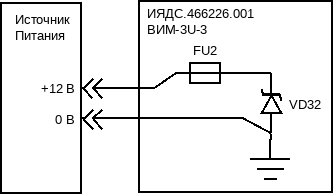
\includegraphics[scale=0.8]{vim_power_adapter_connection_sch.png}} 
\caption{Схема подключения источника питания к плате \DocProductShortTitle~}
\label{ris:vim_power_connection}
\end{figure}

\begin{figure}[!h]
\center{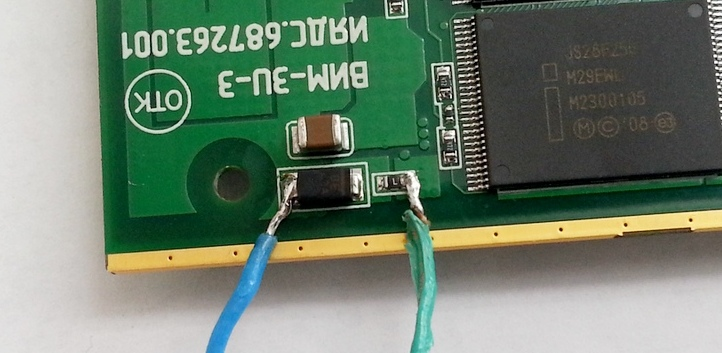
\includegraphics[width=1\linewidth]{vim_vcc12_adapter_solder_foto.jpg}} 
\caption{Фотография места пайки при подключении источника питания к плате \DocProductShortTitle~}
\label{ris:vim_vcc12_adapter_solder_foto}
\end{figure}

%%%Технологическая перемычка нужна долько для программирования ПЛИС вне стенда. Исключаем (?временно) этот пункт
%\begin{figure}[!h]
%\center{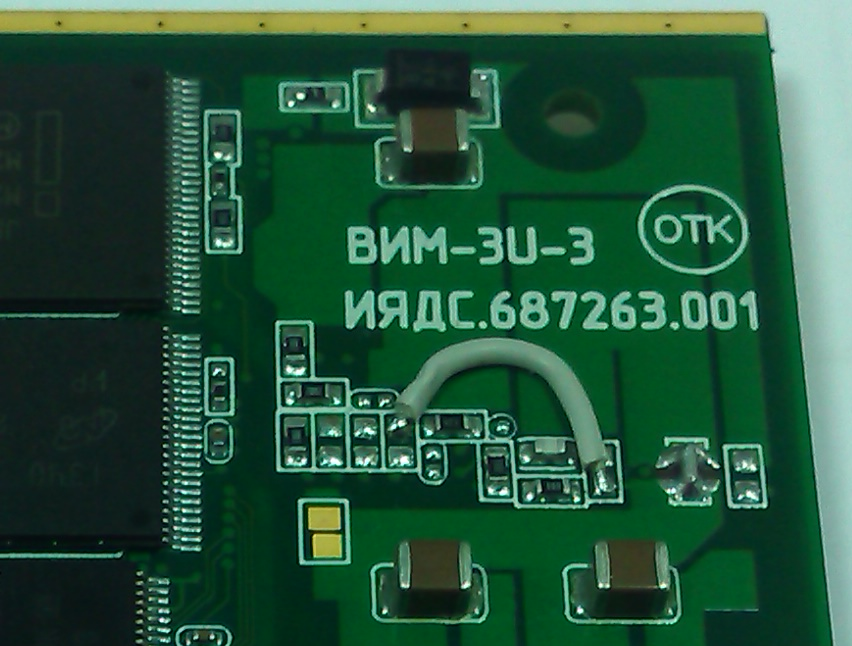
\includegraphics[width=1\linewidth]{vim_3v3aux_tech_jumper_foto.jpg}}
%\caption{Фотография места установки технологической перемычки на плате \DocProductShortTitle~}
%\label{ris:vim_3v3aux_tech_jumper_foto}
%\end{figure}

%%% ----------------------------Приложение Б---------------------------- %%%
\ESKDappendix{обязательное}{Установка перемычек по цепям питания на плате \DocProductShortTitle~}
\label{appendix:power_jumpers}

\begin{figure}[!h]
\center{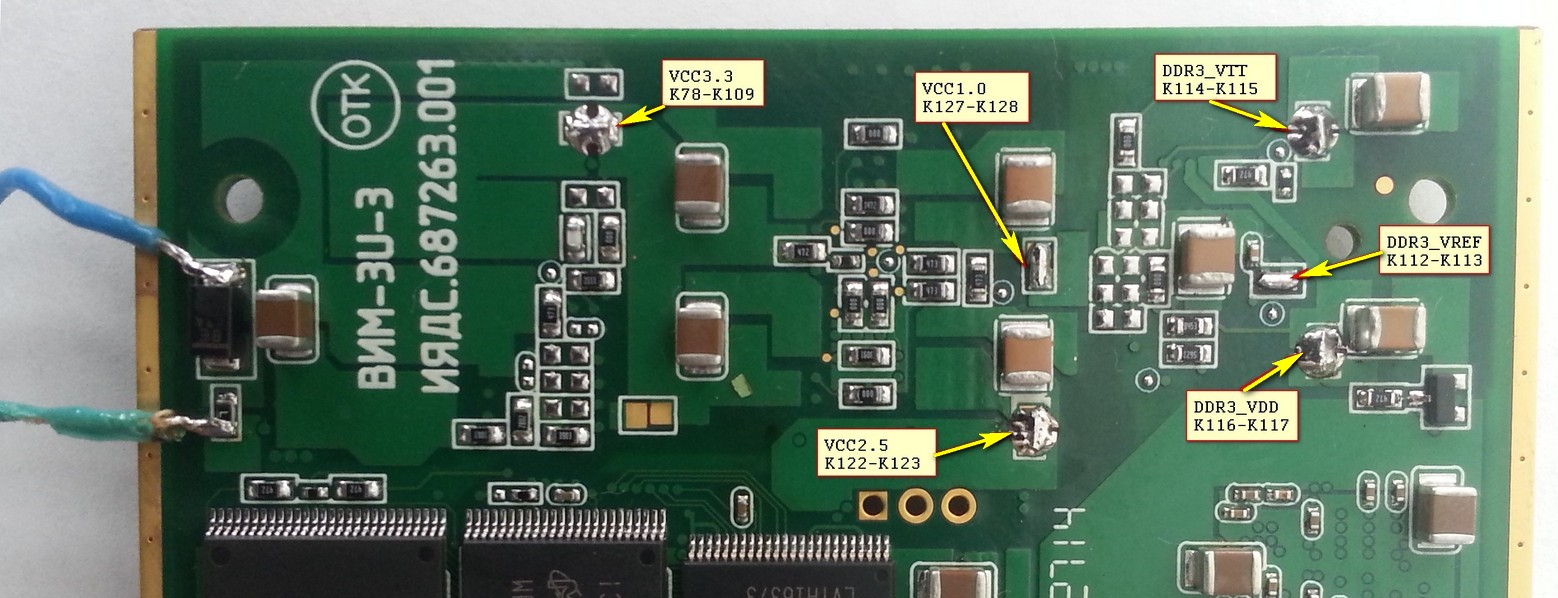
\includegraphics[width=1\linewidth]{vim_power_jumper_foto.jpg}} 
\caption{Фотография установленных перемычек по цепям питания на плате \DocProductShortTitle~}
\label{ris:vim_power_jumper_foto}
\end{figure}

%%% --------------------------------END--------------------------------- %%%


 % Приложения

\newpage % начать с новой страницы

\begin{ESKDchangeSheet}
\rule{0mm}{\textheight-4cm}&&&&&&&&&\\
\end{ESKDchangeSheet}
 % лист регистрации изменений

\end{document}
